% Рабочий перевод бакалаврской работы на русский язык — только для автора.
% Не для сдачи: сдаётся чешский оригинал BachelorThesis.tex.
% Соответствует редакции оригинала от 28.09.2026. Сборка: lualatex + biber
% (latexmk -lualatex prace_ru.tex в этой папке).
\documentclass[a4paper,11pt]{report}

\usepackage[english,russian]{babel}
\babelfont{rm}{Times New Roman}
\babelfont{sf}{Arial}
\babelfont{tt}[Scale=0.88]{Consolas}
\usepackage[a4paper,margin=2.5cm]{geometry}
\usepackage{graphicx}
\graphicspath{{../}}
\usepackage{amsmath}
\usepackage{caption}
\usepackage{tikz}
\usetikzlibrary{fit,arrows.meta}
\usepackage{pgfplots}
\pgfplotsset{compat=1.18}
\usepackage[autostyle=true]{csquotes}
\usepackage[backend=biber,style=numeric,sorting=none]{biblatex}
\addbibresource{../literature.bib}
\usepackage[hidelinks]{hyperref}
\setlength{\emergencystretch}{2em}
\setlength{\parskip}{0.3em}

\title{Переносное устройство для тестирования и мониторинга сетей\\[0.5em]
\large Рабочий перевод бакалаврской работы на русский язык\\
(оригинал: Přenosné zařízení pro testování a monitorování sítí)}
\author{Михаил Муканов\\ VŠB -- Technická univerzita Ostrava, FEI\\ Руководитель: Ing. Pavel Nevlud}
\date{Редакция от 28.09.2026}

\begin{document}

\maketitle

\begin{abstract}
Эта бакалаврская работа посвящена проектированию и реализации переносного устройства для тестирования и мониторинга компьютерных сетей. Устройство построено на одноплатном компьютере Raspberry Pi с сенсорным дисплеем, двумя внешними сетевыми адаптерами и аккумуляторным модулем и управляется без подключённого компьютера. Оба тестовых порта логически разделены пространствами имён ядра Linux, поэтому прибор может одним портом генерировать трафик, а другим независимо его анализировать. Устройство содержит анализатор трафика протоколов IPv4 и IPv6 со статистикой, разбором кадров и фильтрами, которые выполняются в ядре, генератор пакетов, измерение задержки, пропускной способности, потерь и джиттера инструментом iperf3, включая развёртку по размерам кадра, аудит сообщений Router Advertisement и поиск соседей IPv6. Точность анализатора проверена независимым пересчётом захваченного трафика, измерения проведены и на перемычке между портами, и против компьютеров с Linux и Windows. В работе очерчены и пределы использованной платформы, прежде всего пропускная способность, ограниченная шиной USB 2.0 примерно 276 Мбит/с. В типичном режиме прибор работает от аккумулятора почти семь часов.

\medskip
\noindent\textbf{Ключевые слова:} компьютерные сети; мониторинг сети; генерирование трафика; анализатор трафика; Raspberry Pi; network namespaces; IPv4; IPv6; пропускная способность; потери пакетов.
\end{abstract}

\tableofcontents
\listoffigures
\listoftables

\chapter{Введение}
\label{sec:introduction}

Компьютерные сети сегодня — базовая инфраструктура, от надёжности которой зависит работа учреждений и производственных предприятий. С ростом числа подключённых устройств и постепенным внедрением протокола IPv6 наряду с привычным IPv4 растёт и сложность задач, которые администратору сети приходится решать прямо на месте. Вопросы при этом бывают очень конкретными: действительно ли розетка в помещении соединена с распределительным шкафом, какую пропускную способность даёт линия, какие устройства находятся в сегменте и не работают ли на них службы, которых там быть не должно.

Ответ на эти вопросы требует измерения на месте. Именно здесь обычные решения упираются в свои ограничения. Коммерческие ручные тестеры эргономичны, но закрыты: набор их функций задан производителем, и добавить в них собственную методику проверки нельзя. Ноутбук с открытыми инструментами, наоборот, полностью гибок, но в шкафу или под столом с ним работать неудобно, и перед каждым измерением его нужно настраивать вручную. Если же техник попытается подключиться к одному и тому же сегменту двумя интерфейсами, чтобы одновременно слушать трафик и создавать нагрузку, он столкнётся с конфликтом в таблицах маршрутизации операционной системы, который незаметно исказит результаты измерений.

Цель этой бакалаврской работы — спроектировать и реализовать переносное устройство для тестирования и мониторинга компьютерных сетей, которое сочетает открытость программного решения с эргономикой самостоятельного прибора. Прототип построен на одноплатном компьютере Raspberry Pi, оснащён сенсорным дисплеем, собственным управляющим приложением и аккумулятором, поэтому им можно управлять без подключённого компьютера, без физической клавиатуры и без сетевого питания. Он содержит генератор и анализатор трафика, измеряет задержку, пропускную способность, потери и джиттер и позволяет картировать сегмент и проводить разведку безопасности, одинаково для протоколов IPv4 и IPv6.

Ключевой технический элемент конструкции — логическое разделение двух тестовых интерфейсов с помощью технологии Linux Network Namespaces. Это разделение гарантирует, что создаваемая нагрузка не влияет на статистику, захваченную слушающим интерфейсом, и обеспечивается самим ядром операционной системы, а не только аккуратностью оператора при настройке. Второе направление, которому уделено повышенное внимание, — автоматическая настройка адресов в протоколе IPv6, поскольку именно от неё зависит, сможет ли прибор установить связь со станцией, на которой ничего заранее не настроено.

Текст работы разделён на четыре главы. После этого введения следует глава \ref{sec:teorie}, которая излагает теоретические основы: различия протоколов сетевого уровня, адресацию и автоконфигурацию протокола IPv6, генерирование сетевого трафика и измерение его параметров, инструменты мониторинга и аудита трафика и архитектуру пространств имён. Её заключительная часть сравнивает существующие решения и формулирует требования к проектируемому устройству. Глава \ref{sec:realizace} описывает проект прибора с аппаратной и программной стороны, реализацию генератора и анализатора трафика и оценку результатов, проверенных измерениями. Заключение подводит итоги, выделяет собственный вклад автора и намечает направления дальнейшего развития прототипа.

\chapter{Теоретические основы и анализ проблематики}
\label{sec:teorie}

Эта глава посвящена теоретическим основам, на которых построено спроектированное устройство для тестирования и мониторинга. Понимание этих понятий необходимо для правильной интерпретации данных, полученных при анализе сети.

\section{Протоколы сетевого уровня и их различия в производительности}
\label{sec:ipv4_ipv6}

Современные компьютерные сети опираются на сосуществование протоколов IPv4 и IPv6 \cite{nastase2024}. Обе версии выполняют на сетевом уровне одну и ту же задачу — адресацию станций и доставку пакета между сетями, — но различаются настолько, что измерительный прибор должен обслуживать каждую из них отдельно. Одновременная работа обоих протоколов на одном интерфейсе, называемая двойным стеком, сегодня обычна в корпоративных сетях, и переносной анализатор должен уметь проверить работоспособность каждой ветви по отдельности.

Самое заметное различие — длина адреса, выросшая с 32 до 128~бит. Изменение адресного пространства, однако, не единственное вмешательство в конструкцию протокола. Заголовок IPv4 имеет переменную длину от 20 до 60~байт, поскольку за обязательной частью могут следовать дополнительные поля, и содержит, помимо прочего, собственную контрольную сумму и три поля для фрагментации. Заголовок IPv6, напротив, фиксирован и занимает 40~байт \cite{rfc8200}. Вся дополнительная функциональность перенесена в заголовки расширения, которые выстраиваются цепочкой за основным заголовком и на существование которых указывает поле Next Header.

У такой конструкции два следствия, которые проявляются именно при измерениях. Во-первых, маршрутизатор на пути пакета выполняет меньше работы: он не пересчитывает контрольную сумму, потому что её вообще убрали из заголовка, полагаясь на защиту канального и транспортного уровней, и не фрагментирует. Фрагментировать в IPv6 может только отправитель, который для этого должен заранее выяснить наименьший размер передаваемого блока на всём пути. С этим связано требование, чтобы каждая линия передавала пакет размером не менее 1280~байт. Во-вторых, IPv6 полностью отказался от широковещательной рассылки и заменил её групповой, что прямо отражается на том, как устройства в сегменте находят друг друга; этому посвящён подраздел \ref{sec:ipv6_adresace}.

С точки зрения измерения пропускной способности существенно, что вдвое больший основной заголовок — это накладные расходы, которые вычитаются из полезной нагрузки. При одинаковом размере кадра канального уровня на данные остаётся на двадцать байт меньше, поэтому измеренная прикладная пропускная способность у IPv6 получается чуть ниже. Как показывают сравнительные измерения Tuifaiga и соавторов \cite{tuifaiga2021}, IPv4 в локальных сетях действительно достигает несколько большей пропускной способности и меньшей задержки, чем IPv6, одинаково в Windows и Linux.

Различие, впрочем, нужно толковать осторожно. Его относительная величина зависит от того, какими блоками передаются данные: у длинных потоков с полноразмерными кадрами это единицы процентов, а у трафика из коротких пакетов может быть заметно больше. Поэтому измеренная разница между протоколами сама по себе говорит не о качестве сети, а о свойствах протокола, и при оценке нагрузочных тестов из главы \ref{sec:realizace} её нужно отличать от реальных неисправностей.

\section{Адресация и автоматическая настройка протокола IPv6}
\label{sec:ipv6_adresace}

Различие между протоколами не ограничивается размером заголовка. Для переносного анализатора важнее другой способ, которым станция вообще получает свой адрес, поскольку от него зависит, сможет ли прибор обратиться к другой стороне без всякой предварительной договорённости с её владельцем. Поэтому этому вопросу посвящён отдельный подраздел.

Адрес IPv6 имеет длину 128~бит, его структура определена архитектурой адресации \cite{rfc4291}, а сам протокол — документом \cite{rfc8200}. Запись делится на восемь групп по четыре шестнадцатеричные цифры, причём самый длинный непрерывный участок нулевых групп можно заменить двумя двоеточиями. Для тестового устройства важны три категории адресов. Адрес локального канала из диапазона \texttt{fe80::/10} возникает на каждом интерфейсе автоматически в момент поднятия линии и действует только в пределах одного физического сегмента. Глобальный адрес маршрутизируется во всём Интернете. Между ними стоят уникальные локальные адреса, которые для нашего устройства интереснее всего.

Уникальные локальные адреса задаются префиксом \texttt{fc00::/7}, причём восьмой бит различает способ выделения; при его установке, то есть для префикса \texttt{fd00::/8}, организация сама генерирует сорокабитный идентификатор псевдослучайным образом \cite{rfc4193}. Такой префикс с очень высокой вероятностью уникален, не маршрутизируется в Интернете и не зависит ни от какого провайдера. Именно эти свойства соответствуют природе переносного анализатора, который работает в закрытом тестовом сегменте, не имеет постоянного подключения к Интернету и чей адресный план не должен конфликтовать с адресами сети, куда прибор временно подключён.

Вторую половину адреса образует идентификатор интерфейса длиной 64~бита. Один из способов его получения, описанный в архитектуре адресации \cite{rfc4291}, исходит из физического адреса интерфейса и называется EUI-64. Сорокавосьмибитный адрес делится на две половины, между которыми вставляются два байта со значением \texttt{fffe}, а в первом байте инвертируется седьмой бит, различающий универсальное и локальное управление. Так физический адрес \texttt{00:e0:4c:68:02:16} даёт идентификатор \texttt{02e0:4cff:fe68:0216}. Для нашего устройства это практически важно: адрес другой стороны получается детерминированно, и его можно вычислить, а не прописывать жёстко в управляющем приложении.

У идентификатора, полученного из физического адреса, есть, однако, недостаток: он выдаёт оборудование станции и позволяет следить за ней, в какую бы сеть она ни подключилась. Поэтому современные операционные системы чаще используют идентификатор, который для данной сети постоянен, но из физического адреса не выводится \cite{rfc7217}, а рядом с ним ещё и временные адреса, которые регулярно меняются \cite{rfc8981}. Одна станция поэтому обычно несёт на одном интерфейсе несколько адресов сразу и, если так настроена, для исходящей связи предпочитает временный \cite{rfc8981}. Для измерительного прибора отсюда следует, что другая сторона может отвечать не с того адреса, к которому к ней обратились, — в практической части это оказалось существенным.

Обнаружением соседей на общей линии в IPv6 занимается механизм Neighbor Discovery \cite{rfc4861}, который заменяет протокол ARP из IPv4 и построен поверх ICMPv6. С его помощью устройства узнают физические адреса друг друга, проверяют достижимость соседей и находят маршрутизаторы в сегменте. Для нашего устройства ключевые два его сообщения. Сообщением Router Solicitation, отправляемым на групповой адрес всех маршрутизаторов, станция после поднятия интерфейса спрашивает, есть ли в сегменте маршрутизатор. Ответом служит сообщение Router Advertisement, которым маршрутизатор объявляет себя и вместе с тем префиксы, действующие в сегменте. Частью механизма является и обнаружение дублирующихся адресов, которым станция проверяет, что выбранный ею адрес в сегменте ещё не занят.

На сообщении Router Advertisement построена автоконфигурация адресов без сохранения состояния \cite{rfc4862}. Станция сама составляет полный адрес из объявленного префикса и собственного идентификатора интерфейса, без какого-либо сервера, который вёл бы учёт выдачи. Воспользуется ли она этой возможностью и как, определяют три флага в сообщении, значение которых сведено в таблице \ref{tab:priznaky}.

\begin{table}[htbp]
    \caption{Значение флагов в сообщении Router Advertisement}
    \label{tab:priznaky}
    \centering
    \begin{tabular}{clp{7.5cm}}
        \hline
        Флаг & Название & Значение для станции \\
        \hline
        M & Managed address configuration & адрес станция запрашивает у сервера DHCPv6 \\
        O & Other configuration & прочие данные, например адреса DNS, получает от сервера DHCPv6 \\
        A & Autonomous address configuration & из этого конкретного префикса станция может составить адрес сама \\
        \hline
    \end{tabular}
\end{table}

Принципиально, что флаги M и O относятся ко всему сообщению, а флаг A передаётся у каждого объявленного префикса отдельно. Маршрутизатор может в одном сообщении объявить несколько префиксов и для каждого решить, может ли станция вывести из него адрес самостоятельно. Оба пути не исключают друг друга и на практике обычно комбинируются, так что у станции может быть одновременно адрес, составленный без сохранения состояния, и адрес, выданный сервером.

Альтернативой с сохранением состояния является DHCPv6 \cite{rfc8415}, перенимающий роль, знакомую по IPv4: сервер ведёт учёт выданных адресов, привязывает их к идентификатору клиента и управляет сроком аренды. Ценой этого учёта он даёт администратору полный контроль над тем, какая станция какой адрес получит, и позволяет передать и другие параметры настройки.

Разница подходов для переносного тестового устройства существенна. Станция с IPv4 без работающего клиента DHCP адрес не получит никогда, потому что другого механизма протокол не предлагает. Ядро же операционной системы с IPv6 выдаёт адрес локального канала само, а при поднятом флаге A составит из объявленного префикса и адрес более широкой области действия, причём на станции не должна работать никакая служба настройки сети. Анализатор, правильно объявляющий префикс, может поэтому установить связь и с машиной, на которой ничего не настроено и над которой у оператора прибора нет никакого контроля. Проверка этого предположения на собранном прототипе описана в подразделе \ref{sec:overeni_autokonfigurace}.

\section{Генерирование сетевого трафика}
\label{sec:generovani}

Работу с сетевым трафиком можно разделить на два принципиально разных подхода. Пассивный мониторинг только наблюдает трафик и ничего в сеть не отправляет, а активное измерение само создаёт трафик и смотрит, как с ним справится сеть. Переносной анализатор должен уметь и то, и другое, потому что они отвечают на разные вопросы: пассивное наблюдение показывает, что в сегменте происходит на самом деле, активное измерение — на что сегмент способен. Этот раздел посвящён активной стороне, то есть генерированию трафика, следующий — пассивной.

Смысл генерирования в том, что в сеть отправляют трафик с известными свойствами и на приёмной стороне выясняют, что из него и как дошло. Из сравнения отправленного и принятого определяются основные параметры сети. Пропускная способность показывает, сколько данных в секунду сеть передаст. Потери показывают, какая доля отправленных пакетов не дошла. Задержку чаще всего измеряют как время оборота, то есть время между отправкой сообщения Echo Request протокола ICMP и приходом ответа, как это делает утилита ping. Наконец, джиттер (разброс задержки) описывает, насколько колеблется время передачи последовательных пакетов.

Генераторы трафика по уровню, на котором они работают, делятся на две группы. Генераторы потоков создают непрерывную передачу данных между клиентом и сервером и оценивают результаты на обеих сторонах соединения. Типичный представитель — инструмент iperf3 \cite{iperf3}. Выбор транспортного протокола определяет, что именно измеряется. Измерение поверх TCP даёт пропускную способность, достижимую для приложения, с учётом управления потоком и восстановления после потерь, поэтому результат отражает поведение реальной передачи данных. Измерение поверх UDP, наоборот, отправляет с заранее заданной скоростью без оглядки на состояние сети и кроме пропускной способности говорит о потерях и джиттере. Различие между передачей с установлением соединения и без него на высоких скоростях подробно разбирают Gál и соавторы \cite{gal2021}; их работа служит методической основой для измерений в этой работе. Для содержательного результата тест должен длиться достаточно долго, чтобы управление потоком успело установиться, и измерение нужно повторять.

Вторую группу составляют генераторы пакетов, которые собирают отдельные кадры выбранного типа слой за слоем. Они служат не столько для измерения пропускной способности, сколько для проверки, пройдёт ли определённый вид трафика через сегмент и как на него отреагируют остальные устройства. В языке Python для этого есть библиотека Scapy, которая позволяет сложить кадр из отдельных заголовков, отправить его и обработать ответы \cite{carter2024}. В коммерческих тестерах для той же цели стоит специализированная аппаратура, способная отправлять точно рассчитанные по времени кадры на полной скорости линии; программный генератор на обычном компьютере ограничен производительностью процессора и точностью таймеров операционной системы.

Скорость генерируемого трафика можно выразить двумя способами — в битах в секунду и в кадрах в секунду, — и эти величины не взаимозаменяемы. Обработка каждого кадра требует и в сетевом устройстве, и в компьютере определённой постоянной работы независимо от его размера. Поэтому на коротких кадрах устройство обычно исчерпывает свою производительность раньше, чем заполнит пропускную способность линии, и его предел задаётся числом кадров в секунду; на длинных кадрах, наоборот, раньше упирается в пропускную способность линии или шины. Методика измерения производительности сетевых устройств \cite{rfc2544} поэтому предписывает повторять измерение для ряда размеров кадра, для Ethernet это 64, 128, 256, 512, 1024, 1280 и 1518~байт, и пропускной способностью считает наибольшую скорость, при которой не теряется ни один кадр. Для IPv6 рекомендуются те же размеры кадра \cite{rfc5180}, но с оговоркой, что заголовок IPv6 на двадцать байт длиннее и самые короткие кадры могут не вместить все заголовки и данные измерительного инструмента.

Джиттер для UDP обычно оценивают способом, заимствованным из протокола RTP \cite{rfc3550}. Для каждой пары последовательно принятых пакетов определяют разность $D$ между разностью времён их прихода и разностью времён их отправки. Из этих разностей непрерывно вычисляется сглаженная оценка
\begin{equation}
    J_i = J_{i-1} + \frac{|D_{i-1,i}| - J_{i-1}}{16}.
    \label{eq:jitter}
\end{equation}
Поскольку используются только разности времён, часы отправителя и получателя не обязаны быть синхронизированы. По той же формуле считает джиттер и iperf3 \cite{iperf3}. Для толкования результатов полезно также различать среднюю и мгновенную скорость: программный генератор может выдерживать заданную среднюю скорость и при этом отправлять короткими пачками на полной скорости линии, которые принимающее устройство с небольшим буфером может не успеть обработать.

Активное измерение нагружает сеть, поэтому важно, где оно проводится. Методы \cite{rfc2544} разрабатывались для измерения отдельных устройств в изолированной лабораторной среде. Дополняющий документ \cite{rfc6815} прямо предостерегает от их применения в рабочей сети: тестовый трафик может перегрузить ресурсы, общие с пользователями, а результаты к тому же будут неверными, потому что потери от чужого трафика не отличить от потерь измеряемого устройства. Переносной прибор поэтому должен ограничивать нагрузочные тесты закрытым тестовым сегментом.

\section{Мониторинг и аудит безопасности сетевого трафика}
\label{sec:monitorovani}

Пассивный захват в системах на базе Linux построен на библиотеке libpcap и механизме фильтрации в ядре, называемом BPF \cite{mccanne1993}. Программа передаёт ядру фильтр, записанный выражением, например \texttt{tcp} или \texttt{host 10.0.1.20}, и ядро по нему отбрасывает неинтересные кадры ещё до того, как скопирует их в память приложения. Это заметно снижает нагрузку на процессор, что для одноплатного компьютера существенно. Чтобы интерфейс принимал и кадры, адресованные не ему, его нужно перевести в неразборчивый (promiscuous) режим. Поверх этого слоя работает tcpdump, который выводит захваченный трафик или сохраняет его в файл формата pcap для последующего разбора. Главное ограничение пассивного прослушивания — топология современных сетей: коммутатор доставляет кадры только на тот порт, где находится адрес назначения, поэтому анализатор захватит либо трафик, адресованный ему самому, либо трафик на зеркальном порту, либо на линии, в которую он включён напрямую. Это нужно помнить при толковании измеренной статистики.

Из захваченного трафика составляются сводные статистики. Анализатор Wireshark предлагает, в частности, разбивку трафика по протоколам, обзор общающихся станций с объёмом отправленных ими данных и распределение размеров пакетов \cite{wiresharkstat}. Для быстрой диагностики в поле полезнее всего число кадров и бит в секунду, средний размер кадра, доли отдельных протоколов и станции с наибольшим объёмом трафика: они отвечают на вопросы, общается ли в сегменте что-нибудь, какой трафик преобладает и кто его создаёт.

У самого захвата тоже есть пределы. Если программа не успевает обрабатывать кадры так быстро, как они приходят, заполняется буфер в ядре, и дальнейшие кадры ядро выбрасывает. Статистика тогда выглядит правдоподобно, но неполна. К счастью, ядро ведёт счёт выброшенных кадров, так что надёжный анализатор должен указывать это число при каждом измерении. Предел анализатора, как и у генератора, определяется скорее числом кадров в секунду, чем объёмом данных.

Для картирования сегмента снова служит Scapy: анализатор рассылает запросы ARP на все адреса выбранного диапазона и по ответам составляет список активных станций с их физическими адресами. Как отмечает Carter \cite{carter2024}, именно автоматизация таких задач на Python существенно расширяет возможности сетевого аудита, потому что позволяет подстроить собственные методики под конкретную среду.

Ещё одну группу образуют инструменты активной разведки безопасности, среди которых особое место занимает сканер Nmap. Его работа идёт в несколько этапов. Сначала он выясняет, какие адреса выбранного диапазона отвечают, затем у найденных станций исследует состояние выбранных портов и, наконец, по виду ответов пытается определить, какие службы на них слушают и какая операционная система установлена. Последняя задача, называемая снятием отпечатка стека, основана на мелких различиях в том, как разные реализации строят ответы на необычные комбинации флагов.

С активной разведкой неразрывно связан вопрос правомерности. Сканировать чужую сеть без согласия её администратора недопустимо, независимо от того, причиняет ли это вред. Проектируемое устройство решает этот вопрос своей конструкцией: оно работает в закрытом тестовом сегменте, который создаёт само и единственным другим участником которого является станция, подключённая кабелем напрямую. Сканирование поэтому никогда не выходит за пределы пространства, очерченного оператором, — это наряду с точностью измерений вторая причина логического разделения, описанного в следующем разделе.

\section{Архитектура Linux Network Namespaces (netns)}
\label{sec:netns_teorie}

Для автономного тестирования на одной физической машине используется технология Linux Network Namespaces (netns). Она обеспечивает логическую изоляцию сетевых ресурсов прямо на уровне ядра ОС. Каждое пространство имён содержит собственные независимые экземпляры сетевого стека: изолированные таблицы маршрутизации, правила межсетевого экрана и отдельные сетевые интерфейсы.

Только что созданное пространство имён полностью пусто и содержит лишь интерфейс обратной петли, к тому же выключенный. Работоспособная сетевая среда появляется только после переноса в него физического интерфейса и его поднятия. Перенесённый интерфейс одновременно исчезает из исходного пространства, так что основная система больше о нём не знает и ничего через него отправить не может.

Изоляция касается всего сетевого стека, а не только интерфейсов. У каждого пространства свои таблицы маршрутизации, своя таблица соседей, свой набор правил пакетного фильтра и свои слушающие сокеты. Два процесса в разных пространствах могут занять один и тот же порт, не мешая друг другу, что удобно для измерительного прибора с несколькими экземплярами одной службы. Команды направляются в нужное пространство вспомогательной утилитой, которая запускает процесс прямо в нём; весь механизм входит в стандартное ядро и не требует никаких надстроек.

Если пространства имён должны, наоборот, общаться, их соединяют парой виртуальных интерфейсов типа veth, которая ведёт себя как воображаемый кабель между ними. В нашем анализаторе нужно ровно противоположное, поэтому такого соединения нет. Следствие: между двумя тестовыми портами нет пути, и трафик одного не попадёт в другой даже по ошибке.

Ту же задачу можно было бы решить иначе. Можно взять два отдельных компьютера, но это противоречит требованию переносимости и повышает цену. Виртуализация добавила бы накладные расходы, которые одноплатный компьютер несёт с трудом. Остаётся маршрутизация по адресу источника или привязка приложения к конкретному интерфейсу; эти решения работают, но изоляция у них — вопрос правильной настройки, и одна ошибка или инструмент, не поддерживающий привязку к интерфейсу, её разрушит. Пространства имён, напротив, обеспечивают разделение на уровне ядра, так что неправильно направленному трафику некуда уйти, и ошибка проявляется сразу и однозначно, а не тихим искажением измеренных значений.

\section{Анализ проблематики и существующих решений}
\label{sec:analyza}

Задачу проверить состояние сетевой розетки, измерить достижимую пропускную способность или выяснить, какие устройства есть в сегменте, на практике решают тремя разными путями. У каждого свои достоинства, и именно из их сравнения вытекает задание этой работы.

Самый распространённый путь — универсальный компьютер с открытыми инструментами. Захват трафика обеспечит tcpdump или Wireshark, нагрузочные тесты — iperf3, разведку сегмента — Nmap. Это решение даёт наибольшую производительность и свободу, потому что измерительной станцией служит полноценный компьютер. Его слабость — эксплуатация. Ноутбук в шкафу или под столом использовать неудобно, для подключения к тестируемой сети ему обычно нужен переходник, и перед каждым измерением приходится вручную задавать адреса и проверять, куда на самом деле пойдёт трафик. Если же техник подключится к одному сегменту двумя интерфейсами, чтобы одновременно слушать и нагружать, он столкнётся с конфликтом таблиц маршрутизации, описанным в разделе \ref{sec:netns_teorie}: операционная система отправит трафик тем интерфейсом, который соответствует маршруту по умолчанию, а не тем, который имел в виду техник.

Второй путь — коммерческие ручные тестеры, предназначенные именно для работы в поле. Они эргономичны, сразу после включения готовы к работе и не требуют знания командной строки. Плата за удобство — закрытость. Набор функций задан производителем, добавить в прибор собственный скрипт или новую методику нельзя, а расширение обычно означает покупку старшей модели. В учебной и лабораторной среде, где важно видеть и то, как измерение проходит на самом деле, закрытая конструкция скорее мешает.

Третий путь, которому посвящена и эта работа, — одноплатный компьютер с открытой операционной системой. Пригодность платформы Raspberry Pi для этой цели подтверждена в литературе. Coşar и Kiran \cite{cosar2018} исследовали именно производительность и измеряли поведение Raspberry Pi при анализе сетевого трафика, включая загрузку процессора и памяти. Tripathi и Kumar \cite{tripathi2018} на той же платформе одновременно запускали систему обнаружения вторжений, ловушку для атакующих и анализатор пакетов, показав, что мощности платы хватает на несколько сетевых служб сразу. Hariawan и Sunaringtyas \cite{hariawan2021} построили аналогичное решение на более новом поколении платы и применили его в домашней сети.

У этих работ общая черта. На первый план в них выходит пассивная сторона задачи — захват, обнаружение и оценка трафика, который возникает в сети независимо от измерительного устройства. Активное создание нагрузки и особенно его отделение от измерительного пути в них центральной роли не играют, как и вопрос, как управлять прибором без подключённого компьютера.

Именно здесь открывается место для задания этой работы. Цель — соединить достоинства обоих крайних подходов: сохранить открытость и расширяемость компьютера с Linux и при этом достичь эргономики ручного тестера. Из сравнения существующих решений вытекают такие требования к проектируемому устройству. Прибор должен позволять одновременно пассивно слушать и активно генерировать трафик, причём обе задачи должны вестись раздельно, чтобы нагрузка не искажала захваченную статистику. Это разделение должно обеспечиваться логически, а не аккуратностью оператора, — для этого служат пространства имён. Управление должно быть возможно прямо на устройстве, без ноутбука и без физической клавиатуры, и прибор должен на время измерений работать от собственного источника энергии. IPv6 должен поддерживаться так же глубоко, как IPv4, включая автоконфигурацию адресов на другой стороне, поскольку именно она решает, сможет ли прибор обратиться к станции, на которой ничего не подготовлено. И наконец, прибор после подключения к чужой сети не должен сам ничего отправлять; активные тесты должны выполняться только по команде оператора, а нагрузочные — только в закрытом тестовом сегменте, как требует \cite{rfc6815}.

Выполнению этих требований посвящена следующая глава.

\chapter{Проект и реализация, оценка результатов}
\label{sec:realizace}

Эта глава описывает практическую часть работы в том порядке, в каком создавался прототип: от физического проекта прибора и его питания через программную архитектуру и реализацию генератора и анализатора трафика до оценки результатов, проверенных измерениями. Все приведённые значения измерены на собранном прототипе; там, где измерение повторялось в разных схемах подключения, схема всегда указана, потому что от неё результат существенно зависит.

\section{Проект переносного устройства}
\label{sec:navrh_zarizeni}

В качестве вычислительного блока выбран одноплатный компьютер Raspberry Pi 3 Model B+. На плате стоит четырёхъядерный процессор Cortex-A53 с частотой 1,4~ГГц, 1~ГБ оперативной памяти, четыре порта USB 2.0 и беспроводной интерфейс для диапазонов 2,4 и 5~ГГц \cite{rpi3bplus}. Платформа нативно поддерживает операционные системы на базе Linux, что необходимо для работы с пространствами имён и сетевыми инструментами, а её цена соответствует замыслу создать доступную альтернативу коммерческим тестерам.

Выбор платформы несёт ограничение, которое нужно знать заранее, потому что оно прямо ограничивает ценность измерений пропускной способности. Встроенный Ethernet хоть и гигабитный, но подключён к процессору через шину USB 2.0, и производитель указывает для него наибольшую достижимую пропускную способность 300~Мбит/с \cite{rpi3bplus}. На той же шине сидят все порты USB, а значит, и внешние адаптеры, описанные далее. Поэтому прибор не может проверить, передаст ли линия полную гигабитную скорость; его задача — подтвердить работоспособность соединения, измерить пропускную способность в пределах платформы и сравнить протоколы в одинаковых условиях.

Отображение и управление обеспечивает пятидюймовый сенсорный дисплей с разрешением 800 на 480 точек. Изображение передаётся по HDMI, питание дисплея и данные сенсорного слоя идут через контакты GPIO, причём разъём дисплея занимает контакты 1--26. Сенсорный слой резистивный, в системе его обслуживает драйвер ADS7846. Таким образом, для работы прибору не нужны монитор, клавиатура и мышь.

Для одновременного и взаимно разделённого прослушивания и генерирования трафика одного встроенного интерфейса недостаточно, поэтому прибор дополнен двумя внешними гигабитными адаптерами USB/LAN на контроллере RTL8153. Первый служит портом мониторинга, второй — портом генерирования трафика. В первой версии прототипа эти интерфейсы получали от ядра имена \texttt{eth1} и \texttt{eth2}, порядок которых зависит от того, в каком порядке система при старте находит устройства на шине USB. При повторных загрузках оказалось, что интерфейсы меняются именами, так что роль мониторинга доставалась то одному, то другому адаптеру. Поэтому имена теперь назначаются по физическому адресу адаптера: порт мониторинга называется \texttt{mon0}, порт генерирования \texttt{snd0}, и так при каждой загрузке. Собранный прототип показан на рисунке \ref{fig:prototyp}.

\begin{figure}[htbp]
    \centering
    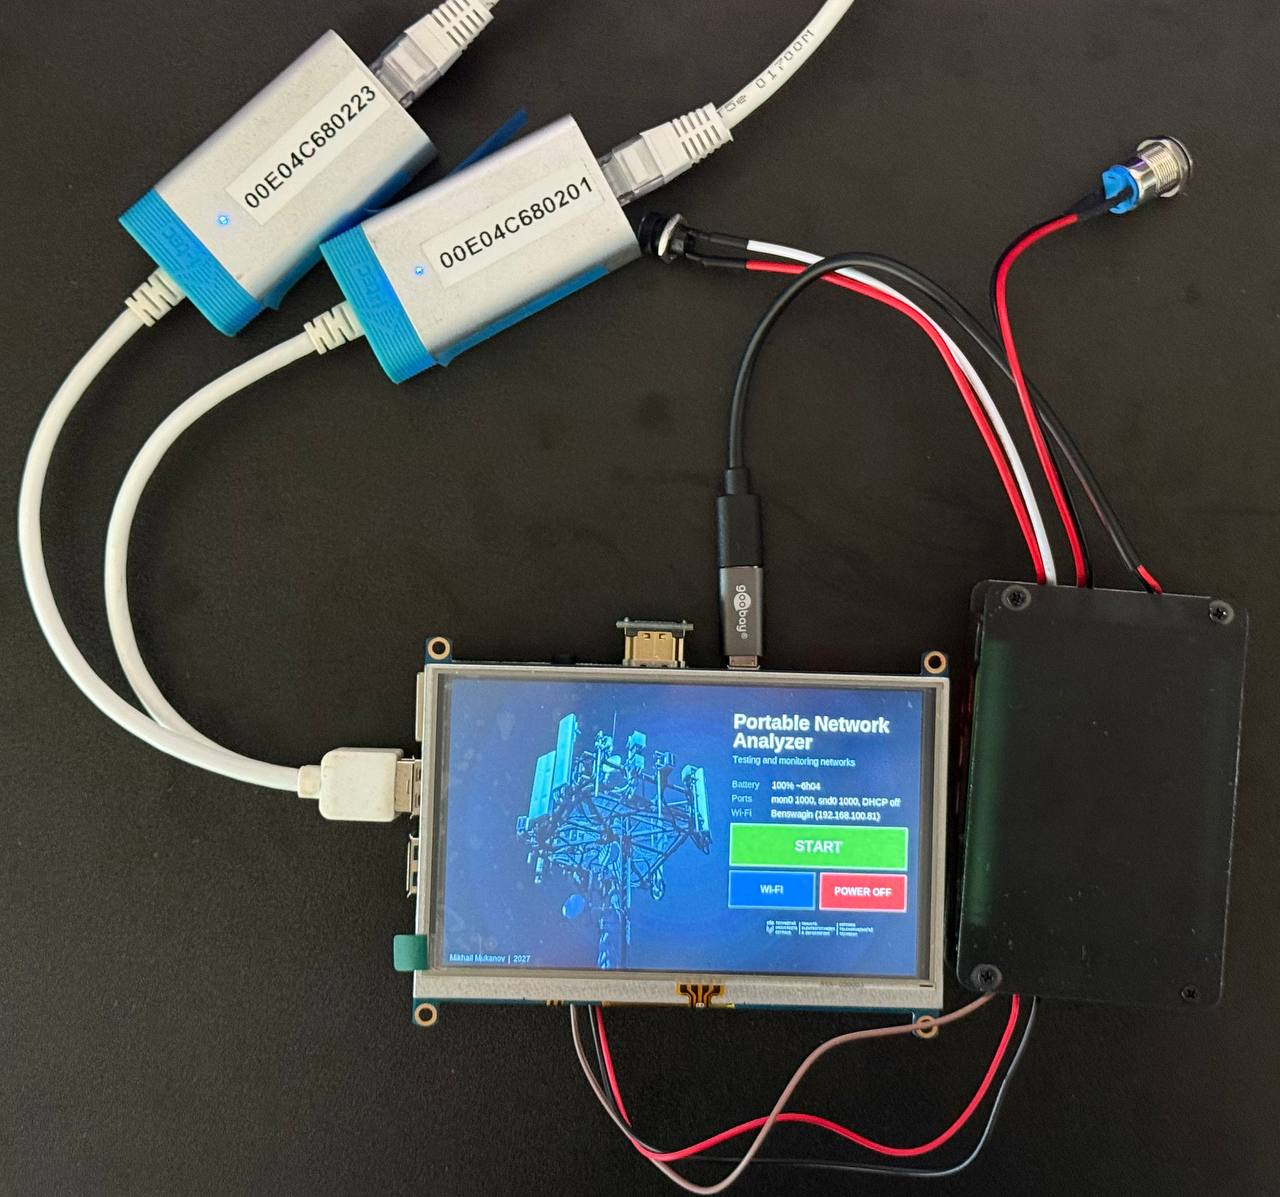
\includegraphics[width=0.75\textwidth]{Figures/device_prototype.jpg}
    \caption[Собранный прототип с аккумуляторным модулем]{Собранный прототип: Raspberry Pi с дисплеем, аккумуляторный модуль, кнопка питания и два подписанных адаптера USB/LAN, соединённых кабелем}
    \label{fig:prototyp}
\end{figure}

\subsection{Питание от аккумулятора}
\label{sec:napajeni}

Переносной прибор должен работать без сетевого источника, поэтому он дополнен аккумуляторным модулем. Выбор модуля ограничила конструкция дисплея. Обычные платы питания для Raspberry Pi подключаются к плате снизу пружинными контактами к GPIO, но разъём дисплея занимает контакты 1--26 с обеих сторон, и плату некуда поставить. Поэтому выбран отдельный модуль Waveshare UPS Module 3S \cite{waveshareups}, который ставится рядом с платой. Модуль несёт три ячейки типа 18650, соединённые последовательно, преобразователь на выходное напряжение 5~В и микросхему INA219 для измерения напряжения и тока ячеек. Установлены ячейки Sony VTC6 ёмкостью 3000~мА·ч. Выход модуля питает Raspberry Pi через её собственный разъём micro-USB, так что дисплей по-прежнему питается от платы.

Ёмкость аккумулятора выбрана по заранее измеренному потреблению прибора. Потребление измерялось USB-тестером, включённым между блоком питания и Raspberry Pi, в шести режимах по десять минут; результаты сведены в таблице \ref{tab:spotreba}. Из измерений следует, что потребление определяется прежде всего объёмом передаваемых данных, а не сложностью выполняемой операции. Сканирование Nmap увеличивает ток по сравнению с простоем всего на 30~мА, пассивное прослушивание на 36~мА, а нагрузочный тест iperf3 на 366~мА.

\begin{table}[htbp]
    \caption{Потребление прибора в разных режимах, измерено на входе 5 В}
    \label{tab:spotreba}
    \centering
    \begin{tabular}{lrr}
        \hline
        Режим работы & Ток [мА] & Мощность [Вт] \\
        \hline
        простой, подсветка дисплея выключена & 678 & 3,40 \\
        простой, подсветка включена & 732 & 3,67 \\
        пассивное прослушивание (типичный режим) & 768 & 3,89 \\
        измерение пропускной способности iperf3 & 1098 & 5,52 \\
        сканирование Nmap & 762 & 3,83 \\
        всё одновременно (худший случай) & 1242 & 6,10 \\
        \hline
    \end{tabular}
\end{table}

Микросхема INA219 подключена к шине I2C. Поскольку контакты обычной шины заняты разъёмом дисплея, шина создана программно на свободных контактах 29--31. Состояние аккумулятора системная служба читает каждые десять секунд, по напряжению определяет оставшийся заряд с помощью кривой разряда, измеренной на этом приборе, и записывает результат в файл, откуда управляющее приложение показывает его в строке состояния. Если напряжение ячеек в трёх измерениях подряд падает ниже 9,6~В, служба штатно выключает прибор, чтобы не повредить ни ячейки, ни файловую систему на карте памяти. Результат разрядного теста приведён в подразделе \ref{sec:overeni_napajeni}.

\subsection{Программная архитектура}
\label{sec:architektura}

Программное обеспечение прибора состоит из управляющего приложения, набора самостоятельных измерительных скриптов и нескольких системных служб. Связи между этими частями показаны на рисунке \ref{fig:architektura}.

\begin{figure}[htbp]
    \centering
    % Блок-схема программной архитектуры (русская версия рис. 3.2)
\begin{tikzpicture}[
    font=\small,
    box/.style={draw, rounded corners=2pt, align=center, minimum height=8mm, inner sep=3pt, fill=white},
    port/.style={draw, thick, align=center, minimum width=16mm, minimum height=7mm, fill=gray!15},
    ns/.style={draw, dashed, rounded corners=4pt, inner sep=5pt},
    lbl/.style={font=\footnotesize\itshape, align=center},
    >=Stealth]

    \node[box, minimum width=38mm] (gui) at (0,0) {управляющее приложение\\(Tkinter, дисплей)};
    \node[box, minimum width=30mm] (sluzby) at (5.2,0.6) {службы systemd:\\порты, состояние\\портов, питание};
    \node[box, minimum width=30mm] (vysledky) at (5.2,-0.8) {каталог результатов\\JSON, CSV, pcap};
    \node[box, minimum width=18mm] (wlan) at (-4.4,0) {\texttt{wlan0}\\Wi-Fi};
    \node[ns, fit=(gui)(sluzby)(vysledky)(wlan)] (vychozi) {};
    \node[lbl, anchor=south west] at (vychozi.north west) {основное пространство имён};

    \node[box, minimum width=40mm] (skripty1) at (-3.2,-3.6) {измерительные скрипты\\(анализатор, ping, iperf3, аудит)};
    \node[port] (mon0) at (-3.2,-5.1) {\texttt{mon0}};
    \node[ns, fit=(skripty1)(mon0)] (nsmon) {};
    \node[lbl, rotate=90, anchor=south] at (nsmon.west) {\texttt{analyzer\_monitor}};

    \node[box, minimum width=40mm] (skripty2) at (3.2,-3.6) {измерительные скрипты\\(генератор, ping, iperf3, аудит)};
    \node[port] (snd0) at (3.2,-5.1) {\texttt{snd0}};
    \node[ns, fit=(skripty2)(snd0)] (nssnd) {};
    \node[lbl, rotate=-90, anchor=south] at (nssnd.east) {\texttt{analyzer\_sender}};

    \coordinate (rozcesti) at (0,-1.9);
    \draw[<->] (gui.south) -- (rozcesti) -| (skripty1.north);
    \draw[<->] (rozcesti) -| (skripty2.north);
    \node[lbl, fill=white] at (rozcesti) {запуск командой \texttt{ip netns exec}\\и возврат строки \texttt{RESULT}};
    \draw[->] (sluzby.west) -- node[lbl, above] {состояние} (sluzby.west -| gui.east);
    \draw[->] (vysledky.west -| gui.east) -- node[lbl, below] {запись} (vysledky.west);

    \draw[thick] (mon0.south) -- ++(0,-0.6) -| node[lbl, pos=0.25, below] {тестируемый сегмент или перемычка между портами} (snd0.south);
\end{tikzpicture}

    \caption{Программная архитектура анализатора и разделение на пространства имён}
    \label{fig:architektura}
\end{figure}

В основе лежит разделение сетевых интерфейсов на пространства имён, описанные в разделе \ref{sec:netns_teorie}. Порт мониторинга принадлежит пространству \texttt{analyzer\_monitor} с адресами \texttt{10.0.1.10/24} и \texttt{fd00:1::10/64}, порт генерирования — пространству \texttt{analyzer\_sender} с адресами \texttt{10.0.2.10/24} и \texttt{fd00:2::10/64}. Управляющее приложение остаётся в основном пространстве, где обслуживает дисплей и беспроводной интерфейс. Между двумя пространствами нет никакого маршрута, в том числе для IPv6: единственный трафик, который попадает с одного порта на другой, — это трафик, прошедший по физическому кабелю.

Из такого устройства вытекает правило, по которому организовано всё программное обеспечение. Каждая функция, которой нужно работать в пространстве одного из портов, — это отдельный скрипт, потому что команда \texttt{ip netns exec} переносит в выбранное пространство весь процесс, а управляющее приложение должно оставаться в основном. Скрипты можно запускать и самостоятельно из командной строки. Свой результат они выводят последней строкой в виде \texttt{RESULT <имя скрипта> <JSON>}, которую управляющее приложение читает и показывает. Каждый такой результат приложение также сохраняет в файл вместе со временем и часовым поясом, признаком того, были ли часы прибора синхронизированы по NTP, и контрольной суммой использованного скрипта. Благодаря этому для каждого измеренного числа можно установить, когда и какой версией программы оно получено.

Пространства имён готовит системная служба, которая запускается всякий раз, когда в системе появляется адаптер с соответствующим физическим адресом, то есть и при загрузке, и при подключении адаптера на ходу. Служба создаёт пространство, если его ещё нет, переносит в него интерфейс, назначает адреса и поднимает линию. Пространство после отключения адаптера сохраняется, так что снова подключённый адаптер возвращается в то же пространство. Вторая служба следит за изменениями состояния линий и адресов в обоих пространствах и записывает их в файл состояния, из которого управляющее приложение читает состояние портов без прав администратора.

Прибор работает в так называемом режиме прибора. После включения без рабочего стола операционной системы сразу запускается управляющее приложение, примерно через 36 секунд после старта ядра. Через десять минут без касаний экран блокируется и гаснет, что экономит 0,35~Вт; подсветка дисплея управляется только механическим переключателем, программно её не погасить.

Особое внимание уделено тому, что прибор сам отправляет в сеть. Переносной прибор может оказаться в чужой рабочей сети и не должен в ней ничего нарушить. Поэтому после подключения кабеля он ничего не отправляет: ядру запрещено самостоятельно искать маршрутизатор сообщением Router Solicitation, сервер dnsmasq, раздающий адреса, запускается только кнопкой, а каждый активный тест — только по команде оператора. Даже с включённым dnsmasq прибор не выдаёт себя за шлюз по умолчанию. Сервер выдаёт подключённой станции только адрес, без параметров шлюза и сервера DNS \cite{rfc2132}, а сообщения Router Advertisement несут нулевое время жизни маршрутизатора, что по \cite{rfc4861} означает, что станция не включит отправителя в список маршрутизаторов по умолчанию. Причина выяснилась при подключении ноутбука с Windows: тот отдаёт проводному интерфейсу приоритет над беспроводным, и если бы анализатор объявил шлюз по умолчанию, ноутбук отправлял бы через него весь трафик в Интернет, куда прибор ничего не пересылает. Так ноутбук сохраняет подключение через Wi-Fi, а с анализатором общается только в пределах тестируемого сегмента.

\section{Реализация генератора и анализатора трафика}
\label{sec:realizace_generatoru}

\subsection{Пользовательский интерфейс}
\label{sec:dotykove_ovladani}

Управляющее приложение написано на Python с библиотекой Tkinter и работает в полноэкранном режиме. Главный экран разделён на двенадцать плиток, каждая из которых открывает одну функцию прибора (рисунок \ref{fig:gui_home}). На плитке после выполнения теста показывается его последний результат, так что оператор видит состояние прибора, не открывая отдельные экраны. Серым отмечены функции, которые ещё в разработке.

\begin{figure}[htbp]
    \centering
    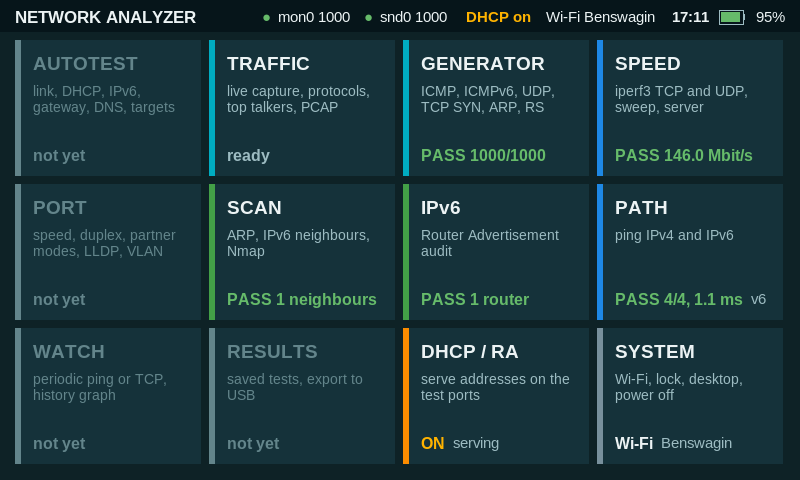
\includegraphics[width=0.72\textwidth]{Figures/gui_home.png}
    \caption{Главный экран управляющего приложения с результатами последних тестов}
    \label{fig:gui_home}
\end{figure}

Все экраны функций устроены одинаково. Вверху строка состояния со временем, состоянием аккумулятора, состоянием линии и скоростью обоих портов, состоянием сервера DHCP и подключением Wi-Fi. Под ней строка итога, которая одним словом PASS, WARN или FAIL и ключевым числом подытоживает последний тест, причём цвет итога всегда дублируется словом. Внизу ряд кнопок с выбором порта, кнопками действий и кнопкой «назад», всегда на одном и том же месте.

Раскладка подчинена резистивной сенсорной панели. Такая панель распознаёт только одно касание, и точность её хуже всего у краёв рабочей области. Поэтому основные кнопки имеют размер не менее 80 на 80 точек, что на этом дисплее соответствует примерно одиннадцати миллиметрам, между соседними элементами промежуток не менее восьми точек, и ни один элемент управления не лежит ближе пятнадцати точек к краю. Соблюдение этих правил на всех экранах проверяет вспомогательный скрипт, который обходит все экраны и измеряет положение и размер каждой кнопки. Приложение не использует жесты; списки листаются кнопками. Адреса вводятся в первую очередь выбором из найденных целей, затем цифровой клавиатурой и лишь в крайнем случае, например при вводе пароля сети Wi-Fi, полной клавиатурой на экране.

\subsection{Анализатор трафика}
\label{sec:analyzator}

Пассивный анализ трафика обеспечивает скрипт \texttt{sniff\_stats.py}. Сам захват выполняет tcpdump, который передаёт захваченные кадры скрипту в двоичном формате pcap. Фильтр, которым оператор ограничивает наблюдаемый трафик, передаётся tcpdump как выражение языка BPF и выполняется в ядре \cite{mccanne1993}; кадры, не прошедшие фильтр, до программы вообще не доходят. Скрипт разбирает у каждого кадра заголовки Ethernet, при наличии метку VLAN, IPv4 или IPv6 вместе с цепочкой заголовков расширения, а далее TCP, UDP, ICMP, ICMPv6 или ARP. Библиотека Scapy для разбора не использована, потому что на процессоре этой платы она слишком медленна для непрерывного потока кадров.

Раз в секунду скрипт выводит строку со сводными показателями: число кадров и бит в секунду, средний размер кадра, доли протоколов, соотношение трафика IPv4 и IPv6, число разных станций и пять станций с наибольшим объёмом отправленных данных. Эти показатели соответствуют статистикам анализатора Wireshark \cite{wiresharkstat}. Строка содержит также несколько последних захваченных кадров с их разбором, так что управляющее приложение получает не одно сообщение на каждый кадр, а одно сводное сообщение в секунду. В конце захвата скрипт сообщает, сколько кадров ядро не успело передать и выбросило, так что возможная потеря при захвате измеряется, а не угадывается.

При проверке выяснилось, что на интерфейсах по умолчанию включены функции, которыми сетевая карта и ядро склеивают последовательные сегменты TCP в один большой пакет. Анализатор тогда видел вместо кадров размером не более 1514~байт пакеты в десятки килобайт, и счётчики и средний размер искажались. Поэтому скрипт на время захвата выключает эти функции на наблюдаемом порту и после окончания возвращает их в исходное состояние.

Поверх скрипта построен экран TRAFFIC (рисунок \ref{fig:gui_traffic}). В верхней части он показывает главные показатели, под ними полосу с долями протоколов, слева самые активные станции, справа текущую ленту последних кадров. Кнопка PAUSE останавливает ленту, счёт при этом продолжается, и показывает последние двести кадров постранично. Касание кадра открывает его разбор по слоям; на рисунке \ref{fig:gui_packet_ra} показан разбор сообщения Router Advertisement с флагами и опциями. Кнопка FILTER предлагает предустановки TCP, UDP, ICMP, ARP, DHCP, ND/RA и DNS и фильтр по выбранной станции; выбранная предустановка превращается в выражение BPF, и захват перезапускается с ним. Кнопка SAVE сохраняет захваченный трафик в формате pcap для разбора в Wireshark, ход показателей в формате CSV и сводный результат в формате JSON.

\begin{figure}[htbp]
    \centering
    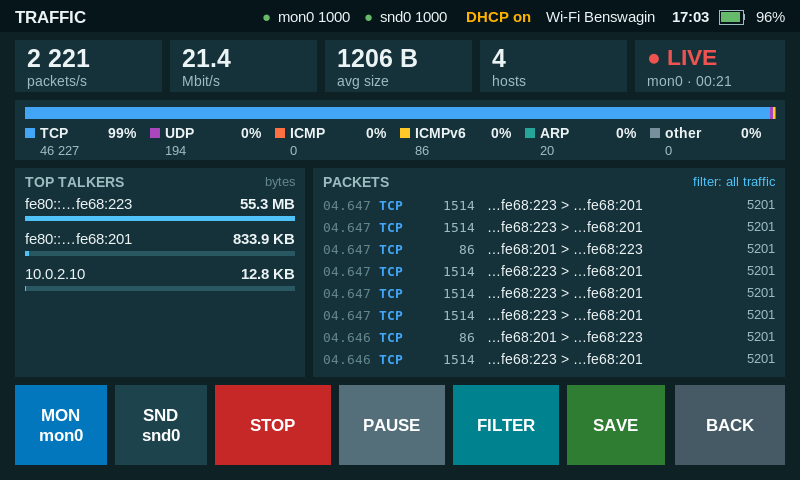
\includegraphics[width=0.72\textwidth]{Figures/gui_traffic.png}
    \caption{Экран TRAFFIC при захвате трафика на порту мониторинга}
    \label{fig:gui_traffic}
\end{figure}

\begin{figure}[htbp]
    \centering
    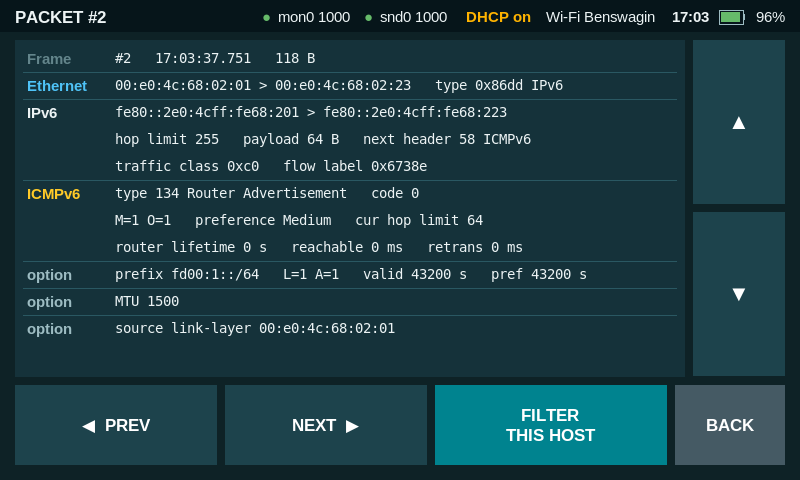
\includegraphics[width=0.72\textwidth]{Figures/gui_packet_ra.png}
    \caption{Разбор захваченного сообщения Router Advertisement по слоям}
    \label{fig:gui_packet_ra}
\end{figure}

\subsection{Генератор пакетов}
\label{sec:generator}

Инструмент iperf3 измеряет пропускную способность, но не позволяет отправить точно заданное число пакетов определённого типа. Для этого служит скрипт \texttt{pkt\_gen.py}. Он умеет собирать сообщения ICMP и ICMPv6 Echo Request, датаграммы UDP, сегменты TCP с флагом SYN, запросы ARP и сообщения Router Solicitation в заданном количестве, с заданной скоростью и размером кадра. Кадры он заранее собирает библиотекой Scapy \cite{carter2024} и отправляет прямо на канальный уровень, так что медленная библиотека в цикле отправки вообще не участвует и скорость ограничена только процессором и шиной. Целью могут быть только адреса тестового стенда; на другие адреса скрипт без явного подтверждения ничего не отправит.

Экран GENERATOR объединяет генератор с анализатором (рисунок \ref{fig:gui_generator}). Пакеты отправляет один порт прибора, а второй порт в собственном пространстве имён считает их анализатором с фильтром по физическому адресу отправителя и выбранному типу пакета. Пакеты, таким образом, заведомо проходят по кабелю из одного пространства имён в другое, и результат сразу сравнивается: равное число отправленных и принятых пакетов даёт итог PASS, разница показывается как потеря.

\begin{figure}[htbp]
    \centering
    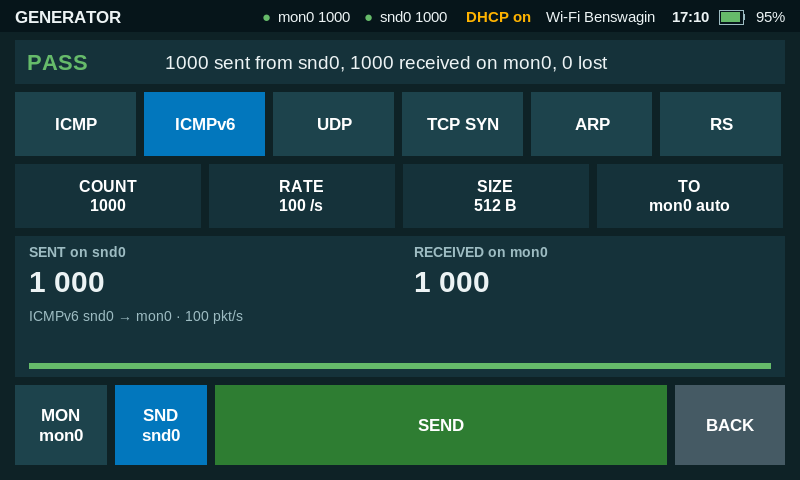
\includegraphics[width=0.72\textwidth]{Figures/gui_generator.png}
    \caption[Генератор пакетов: отправлено портом \texttt{snd0}, посчитано на \texttt{mon0}]{Генератор пакетов: тысяча сообщений ICMPv6, отправленных портом \texttt{snd0} и посчитанных на порту \texttt{mon0}}
    \label{fig:gui_generator}
\end{figure}

\subsection{Измерение задержки, пропускной способности и потерь}
\label{sec:mereni_realizace}

Задержку и доступность другой стороны измеряет экран PATH тестом ping. Пропускную способность, потери и джиттер измеряет экран SPEED инструментом iperf3. Обоим тестам нужна цель. В первой версии приложения адреса целей были прописаны жёстко, позже их можно было найти кнопкой, описанной в подразделе \ref{sec:vyhledavani_sousedu}. Теперь, если цель не задана, тесты ищут её сами в таком порядке: адрес, который выдал подключённой станции DHCP-сервер прибора, затем соседи, известные ядру, и наконец ответ на сообщение Echo Request, отправленное на групповой адрес всех узлов. Каждый кандидат перед использованием проверяется новым запросом ARP или Neighbor Solicitation, потому что запись о выданном адресе живёт ещё часы после отключения станции. Если прибор по физическому адресу понимает, что ответил его собственный второй порт, он сообщает, что порты соединены между собой.

Если тест не находит цель или цель не отвечает, он сообщает оператору причину и рекомендацию. На перемычке между портами, например, тест по IPv4 объясняет, что порты принадлежат разным подсетям и между ними ничего не маршрутизирует, и советует использовать IPv6 (рисунок \ref{fig:gui_path_loop}). Если станция отвечает на запрос ARP или Neighbor Solicitation, но не на ping, прибор сообщает, что станция подключена, но ping блокирует её межсетевой экран.

\begin{figure}[htbp]
    \centering
    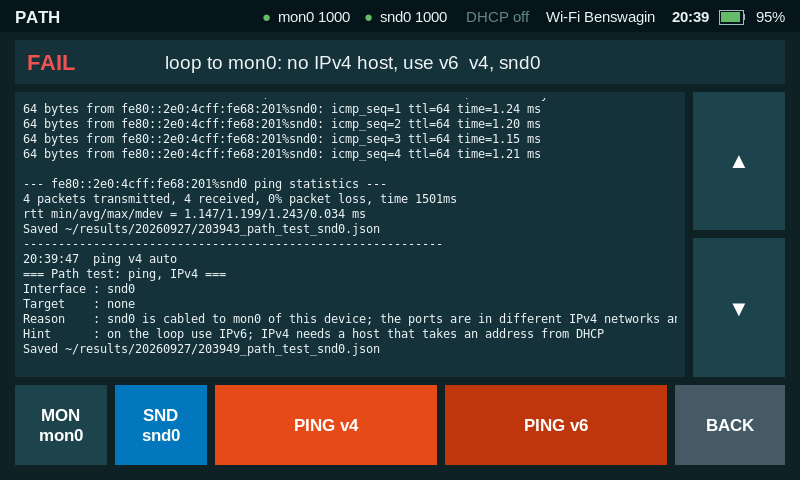
\includegraphics[width=0.72\textwidth]{Figures/gui_path_loop.png}
    \caption[Тест ping на перемычке между портами с объяснением отсутствующей цели]{Тест ping на перемычке между портами: цель IPv6 найдена автоматически, для IPv4 прибор объясняет, почему цели не существует}
    \label{fig:gui_path_loop}
\end{figure}

Нагрузочными тестами управляет скрипт \texttt{perf\_test.py}, который запускает iperf3 \cite{iperf3} с выводом в формате JSON и берёт числа оттуда, а не из текстового вывода. Оператор выбирает протокол TCP или UDP, версию IP, для UDP скорость отправки, длительность теста и направление, то есть кто отправляет данные — анализатор или другая сторона. Для UDP прибор кроме пропускной способности показывает число потерянных датаграмм и джиттер (рисунок \ref{fig:gui_speed_udp}). К каждому результату скрипт записывает среднюю загрузку процессора, температуру чипа в начале и в конце теста и признак того, не притормаживался ли процессор из-за температуры или питания. Измерение с притормаживанием помечается предупреждением, потому что его результат нельзя сравнивать с остальными.

\begin{figure}[htbp]
    \centering
    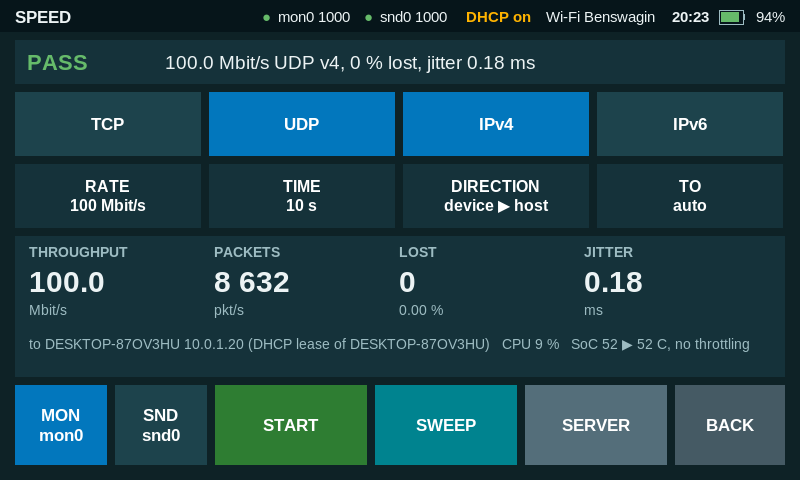
\includegraphics[width=0.72\textwidth]{Figures/gui_speed_udp.png}
    \caption[Измерение по UDP против ноутбука]{Измерение по UDP против ноутбука: пропускная способность, датаграмм в секунду, потери и джиттер}
    \label{fig:gui_speed_udp}
\end{figure}

У экрана SPEED есть ещё две функции. Кнопка SWEEP запускает измерение по UDP последовательно для семи размеров кадра, рекомендованных для Ethernet в \cite{rfc2544}, и показывает результаты таблицей. Размер кадра пересчитывается в размер данных датаграммы отдельно для IPv4 и IPv6, потому что заголовок IPv6 на двадцать байт длиннее. Кадр размером 64~байта для IPv6 собрать нельзя: заголовки Ethernet, IPv6 и UDP вместе с контрольной суммой кадра сами занимают 66~байт, а iperf3 нужно не меньше 16~байт данных. Поэтому ряд для IPv6 начинается с кадра размером 82~байта, что \cite{rfc5180} для измерительных инструментов допускает. Кнопка SERVER, наоборот, запускает на выбранном порту сервер iperf3 и показывает на дисплее адреса, к которым должна подключиться другая сторона; измеряет тогда ноутбук против анализатора. Поскольку методы \cite{rfc2544} не предназначены для рабочих сетей \cite{rfc6815}, измерение против адреса вне тестового стенда прибор запускает только после повторного подтверждения, а развёртку по размерам кадра вне стенда не запускает вовсе. Если цель — второй порт того же прибора, скрипт сам запускает на нём сервер iperf3 на время теста, так что измерение на перемычке не требует никакой подготовки.

\subsection{Автоконфигурация адресов IPv6}
\label{sec:autokonfigurace}

Требование полной поддержки IPv6 при реализации оказалось самой трудной частью настройки — из-за различной природы двух протоколов. Если станция с IPv4 без клиента DHCP получить адрес не может, то IPv6 наряду с сервером DHCPv6 с сохранением состояния предлагает автоконфигурацию без сохранения состояния, при которой станция сама составляет адрес из префикса, объявленного в сообщении Router Advertisement. Какой путь выберет станция, определяет само сообщение: флаг M отсылает её к серверу DHCPv6, а флаг A, передаваемый у каждого префикса отдельно, только разрешает составить адрес из этого префикса \cite{nastase2024}.

Сервер dnsmasq работает в каждом пространстве имён отдельно и обслуживает только интерфейс своего пространства. В первой реализации диапазон адресов IPv6 был записан как один конкретный адрес: \texttt{-{}-dhcp-range=fd00:1::20,fd00:1::20,64,12h}. Это внешне безобидное сужение диапазона привело к тому, что сервер выставил флаги в сообщении Router Advertisement так, как показано в таблице \ref{tab:ra_flags}. Значения считаны на станции утилитой \texttt{rdisc6}, которая запрашивает сообщение и выводит его содержимое.

\begin{table}[htbp]
    \caption{Флаги в сообщении Router Advertisement до и после исправления}
    \label{tab:ra_flags}
    \centering
    \begin{tabular}{lcc}
        \hline
        Флаг & Исходная настройка & После добавления \texttt{slaac} \\
        \hline
        M -- Stateful address configuration & Yes & Yes \\
        O -- Stateful other configuration & Yes & Yes \\
        A -- Autonomous address configuration & No & Yes \\
        On-link & Yes & Yes \\
        \hline
    \end{tabular}
\end{table}

Автоконфигурации мешали, таким образом, сразу два обстоятельства. Поднятый флаг M отсылал станцию к серверу DHCPv6, а опущенный флаг A у префикса запрещал составить из него адрес самостоятельно. dnsmasq выставляет оба именно так, если диапазон задан конкретным адресом, поскольку понимает такую запись как указание раздавать адреса только с сохранением состояния. Решением оказалось добавление ключевого слова \texttt{slaac} в тот же параметр: \texttt{-{}-dhcp-range=fd00:1::20,fd00:1::20,slaac,64,12h}. После этой единственной правки анализатор начал объявлять префикс с поднятым флагом A, не переставая обслуживать запросы с сохранением состояния.

Эффект проявился сразу. Ядро станции составило из объявленного префикса адрес \texttt{fd00:1::2e0:4cff:fe68:216}, помеченный в системном выводе признаком \texttt{proto kernel\_ra}, то есть адрес, созданный самим ядром без участия какого-либо процесса в пространстве пользователя. Идентификатор интерфейса в его второй половине соответствует физическому адресу интерфейса станции \texttt{00:e0:4c:68:02:16}, преобразованному по EUI-64, так что адрес другой стороны вычисляется из её физического адреса.

Из наблюдения следует вывод важнее самого исправления настройки. Различие протоколов не в объёме ручной работы, ведь современные менеджеры сетевых подключений создают профиль сами для обоих протоколов. Различие в том, нужен ли на станции вообще какой-либо процесс: в IPv4 без клиента DHCP адрес не появится никогда, а в IPv6 ядро выдаёт адрес локального канала сразу после поднятия интерфейса и при поднятом флаге A составляет из объявленного префикса и адрес более широкой области действия.

\subsection{Аудит сообщений Router Advertisement}
\label{sec:audit_ra}

Выводы предыдущего подраздела показали, что способ адресации всего сегмента определяет содержимое одного-единственного сообщения. Станция сама не проверяет, кто отправил сообщение Router Advertisement, и примет его от любого, кто пошлёт его в сегмент \cite{rfc4861}. Для диагностического прибора отсюда следует задача уметь это сообщение захватить, разобрать и оценить, соответствует ли оно требованиям стандарта. Эту задачу выполняет скрипт \texttt{ra\_audit.py}, который оператор запускает с экрана IPv6.

Скрипт сначала начинает слушать сообщения ICMPv6, а затем сам отправляет сообщение Router Solicitation на групповой адрес \texttt{ff02::2}, чтобы не ждать периодического объявления. Из захваченных сообщений он извлекает значение Cur Hop Limit, флаги M и O, предпочтение и время жизни маршрутизатора, а из опций — объявленные префиксы с их флагами и временами жизни, значение MTU, адреса серверов DNS и физический адрес отправителя. Над разобранным сообщением он выполняет набор проверок: соответствует ли Hop Limit в заголовке предписанным 255 и является ли адрес источника адресом локального канала \cite{rfc4861}, имеет ли префикс с поднятым флагом A длину 64~бита \cite{rfc4862}, не превышает ли предпочтительное время жизни время действительности, не опускается ли MTU ниже минимума 1280~байт \cite{rfc8200} и совпадает ли физический адрес в кадре с адресом в опции. Каждое сообщение содержит ссылку на соответствующий документ прямо в тексте.

При проверке выяснилось, что делить сообщения только на свои и чужие по физическому адресу отправителя недостаточно, потому что интерфейс захвата видит и кадры, уходящие с того же порта. Прибор поэтому объявлял о присутствии маршрутизатора, когда наблюдал отправку собственного dnsmasq. Происхождение сообщения поэтому различается в три ступени: кадр, отправленный этим же портом; кадр со второго порта того же прибора, пойманный по кабелю; и кадр чужого маршрутизатора — единственный повод для тревоги.

Из того же механизма вытекает ограничение: прибор не может запросить сообщение Router Advertisement у сервера, работающего на этом же порту, потому что запрос уходит прямо на канальный уровень в обход сетевого стека и сервер его не замечает. Сообщение должно пройти по кабелю, поэтому аудит проверяется в схеме, где оба порта соединены одним кабелем; каждый из них тогда слышит объявления другого.

\subsection{Поиск соседей}
\label{sec:vyhledavani_sousedu}

Жёстко прописанные адреса другой стороны годятся на лабораторном стенде, но не в поле, где у подключённого устройства может быть свой адресный план. Вывод о том, что адрес, составленный автоконфигурацией, вычисляется из физического адреса, даёт способ избавиться от этого допущения. Эту функцию обеспечивает скрипт \texttt{neigh\_scan.py}, запускаемый кнопкой NEIGHBORS с экрана SCAN.

Скрипт отправляет сообщение Echo Request на групповой адрес всех узлов \texttt{ff02::1} и дополняет ответы содержимым таблицы соседей ядра. Для каждого найденного физического адреса он вычисляет идентификатор интерфейса по EUI-64 и сравнивает его с адресом локального канала, который сосед реально использует. Совпадение значит, что станция строит идентификатор классически из физического адреса; несовпадение — что она использует идентификатор, не выдающий оборудование, по \cite{rfc7217}, смысл которого — не дать следить за станцией в разных сетях. Если вычисление возможно, скрипт для каждого префикса на порту составляет адрес-кандидат и проверяет его тестом доступности, так что в результат попадает подтверждённый адрес, а не догадка. Той же кнопкой запускается и сканирование ARP в диапазоне адресов порта, так что оператор видит результат обоих протоколов рядом.

\section{Оценка достигнутых результатов}
\label{sec:zhodnoceni}

Прототип проверялся в трёх схемах подключения. Вначале он был проверен в лаборатории компьютерных сетей, где был соединён двумя кабелями со станцией под Linux (рисунок \ref{fig:zapojeni}); такая же схема с персональным компьютером под Linux позже послужила для измерения автоконфигурации. Большая часть дальнейших измерений проведена в схеме, где оба порта прибора соединены одним кабелем между собой. Такое измерение повторяемо и не требует никакого другого оборудования, но прибор в нём измеряет сам себя. Поэтому результаты дополнительно проверены с ноутбуком под Windows 11, к которому оба порта были подключены через два дополнительных адаптера USB/LAN. Эта третья схема выявила несколько обстоятельств, которые перемычка между портами скрывает; они описаны в подразделе \ref{sec:overeni_notebook}.

\begin{figure}[htbp]
    \centering
    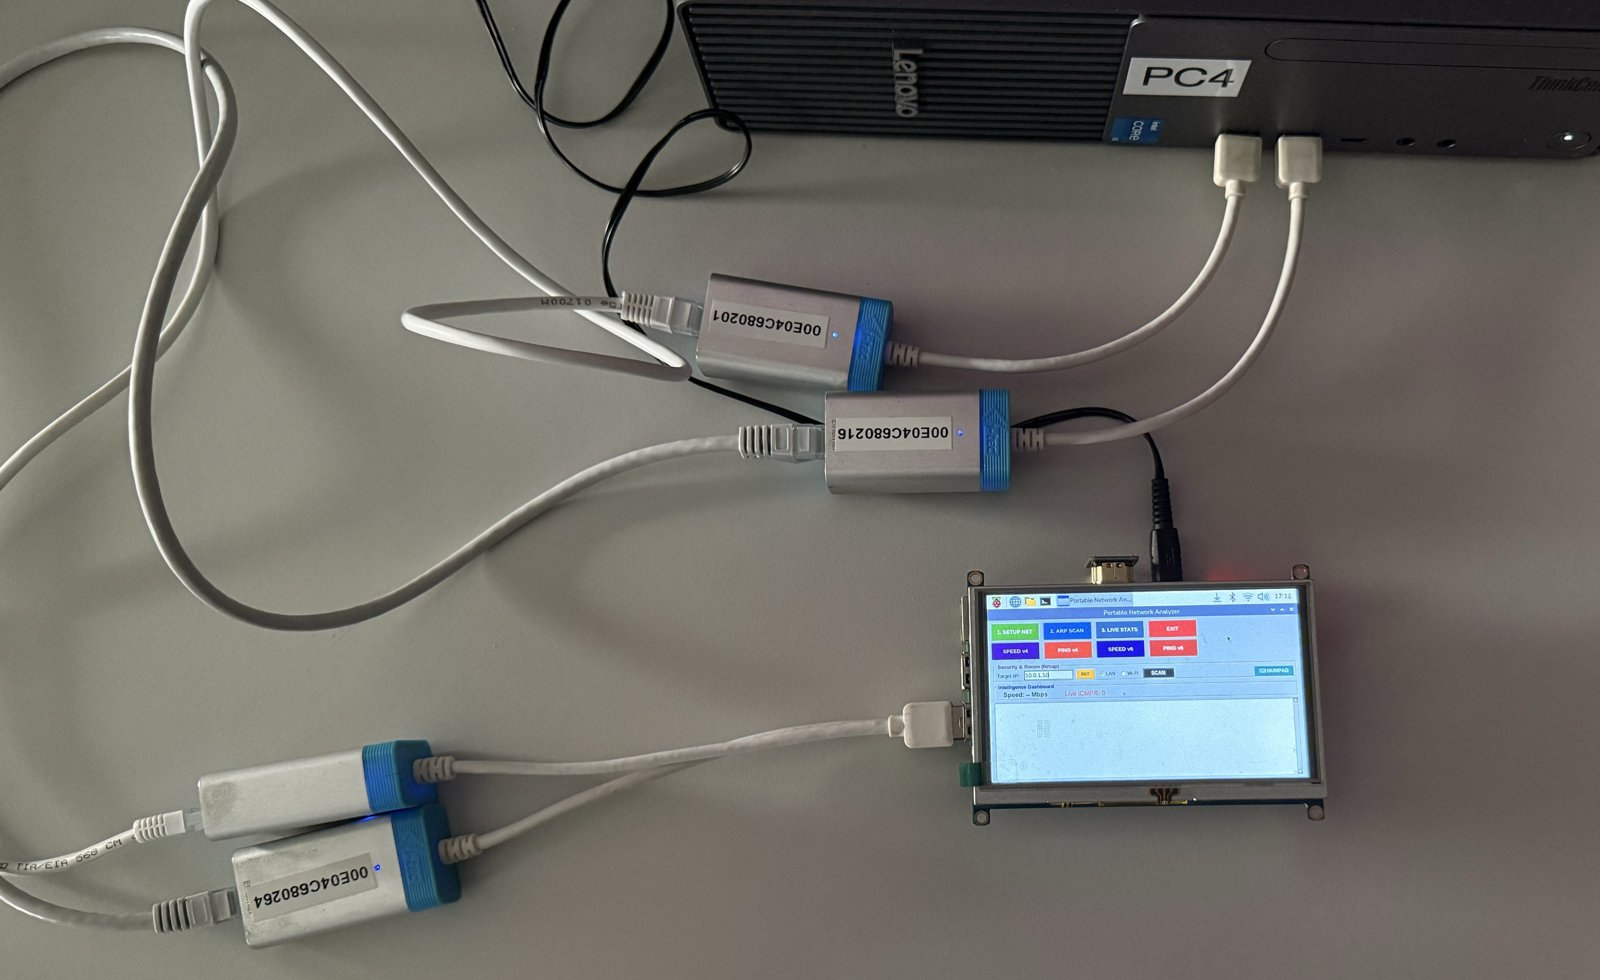
\includegraphics[width=0.75\textwidth]{Figures/lab_connection.jpg}
    \caption{Физическое подключение анализатора к станции в лаборатории}
    \label{fig:zapojeni}
\end{figure}

\subsection{Проверка автоконфигурации адресов}
\label{sec:overeni_autokonfigurace}

Поведение автоконфигурации, описанное в подразделе \ref{sec:autokonfigurace}, проверено измерением, при котором анализатор был соединён со станцией обоими портами сразу. Порт мониторинга перезапущен с добавленным ключевым словом \texttt{slaac}, а порт генерирования оставлен в исходной настройке как контрольный образец. Адреса, выданные обоим интерфейсам станции, сведены в таблице \ref{tab:adresy}.

\begin{table}[htbp]
    \caption{Адреса, выданные станции на обоих тестовых портах}
    \label{tab:adresy}
    \centering
    \begin{tabular}{lll}
        \hline
        Порт анализатора & Адрес станции & Способ получения \\
        \hline
        мониторинг, A = 1 & \texttt{10.0.1.20} & DHCPv4 \\
        мониторинг, A = 1 & \texttt{fd00:1::20/128} & с сохранением состояния, DHCPv6 \\
        мониторинг, A = 1 & \texttt{fd00:1::2e0:4cff:fe68:216/64} & без сохранения состояния, ядром из RA \\
        генерирование, A = 0 & \texttt{10.0.2.20} & DHCPv4 \\
        генерирование, A = 0 & \texttt{fd00:2::20/128} & с сохранением состояния, DHCPv6 \\
        \hline
    \end{tabular}
\end{table}

Суть измерения — разница между двумя строками с IPv6. На порту мониторинга рядом с выданным сервером адресом появился и адрес, составленный ядром из объявленного префикса, а на контрольном порту с опущенным флагом A такого адреса не появилось, хотя оба интерфейса всё время были активны и обслуживались одним устройством. Добавление одного ключевого слова, таким образом, — реальная и единственная причина наблюдаемого изменения. Тесты доступности к адресам, выданным сервером, и к адресу, составленному автоконфигурацией, прошли без потерь с временем отклика около одной миллисекунды.

\subsection{Проверка аудита IPv6}
\label{sec:overeni_auditu}

Аудит проверен на перемычке между портами, где обе линии поднялись на скорости 1000~Мбит/с в полнодуплексном режиме. Разбор сообщения, захваченного на порту \texttt{snd0} после включения dnsmasq, показан на рисунке \ref{fig:gui_ra_audit}. Прибор правильно определил, что объявляющим маршрутизатором является его собственный второй порт, поскольку физический адрес отправителя совпадает с одним из его интерфейсов и сообщение принято по кабелю. Из сообщения он извлёк префикс \texttt{fd00:1::/64} с флагами L и A, время действительности 43\,200 секунд и MTU 1500~байт. Нулевое время жизни маршрутизатора, введённое намеренно (подраздел \ref{sec:architektura}), он оценил лишь как информацию, потому что сообщение исходит от собственного прибора. Он также отметил, что сообщение одновременно несёт флаг M и префикс с флагом A, то есть предлагает станциям и адрес от сервера, и автоконфигурацию; это точное описание поведения dnsmasq после добавления \texttt{slaac}, а не ошибка, и это соответствует таблице \ref{tab:adresy}.

\begin{figure}[htbp]
    \centering
    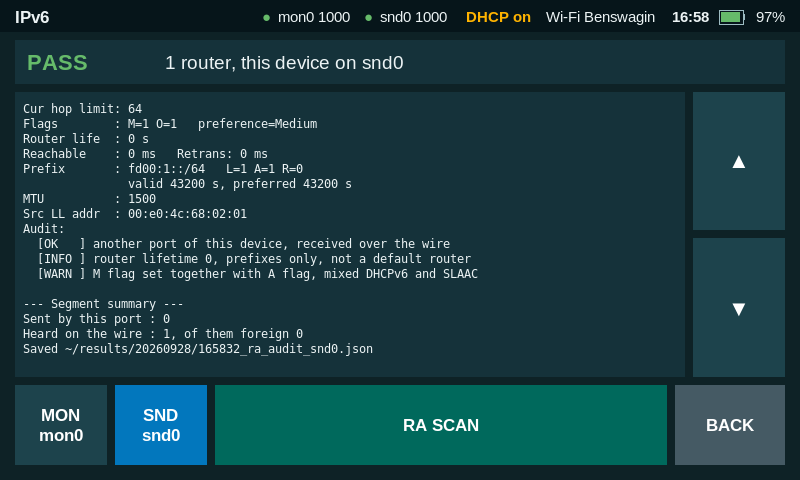
\includegraphics[width=0.72\textwidth]{Figures/gui_ra_audit.png}
    \caption{Аудит сообщения Router Advertisement, принятого от второго порта прибора}
    \label{fig:gui_ra_audit}
\end{figure}

Той же схемой удалось подтвердить таблицу \ref{tab:ra_flags} измерением самого прибора: с исходной настройкой аудит показал у префикса опущенный флаг A и предупреждение, что автоконфигурация запрещена, после добавления \texttt{slaac} — поднятый флаг. Сами проверки на реальном трафике проверить не удалось, потому что в тестируемом сегменте нет неправильно настроенного маршрутизатора. Поэтому они проверены на программно собранном стенде из двух временных пространств имён, соединённых виртуальной парой интерфейсов, куда было вброшено намеренно испорченное сообщение: Hop Limit 64, адрес источника вне локального канала, префикс длиной 48~бит с поднятым флагом A, предпочтительное время жизни больше времени действительности, MTU 1200~байт и другой физический адрес в опции. Прибор отметил все несоответствия сразу и оценил сообщение как сообщение чужого маршрутизатора.

Поиск соседей проверен на той же перемычке (рисунок \ref{fig:gui_neighbours}). Прибор нашёл единственного соседа, вычислил из его физического адреса идентификатор интерфейса, установил совпадение с адресом локального канала и для обоих префиксов на порту составил адрес, который проверил как достижимый. Нагляднее всего, однако, сравнение обоих протоколов в один и тот же момент, сведённое в таблице \ref{tab:sousede}. Сканирование ARP не нашло никого, потому что порты находятся в разных подсетях и на другом конце не работает клиент DHCP. IPv6 на том же кабеле нашёл того же соседа и проверил его адрес, без единого процесса настройки. Утверждение из подраздела \ref{sec:autokonfigurace} подкреплено, таким образом, измерением.

\begin{figure}[htbp]
    \centering
    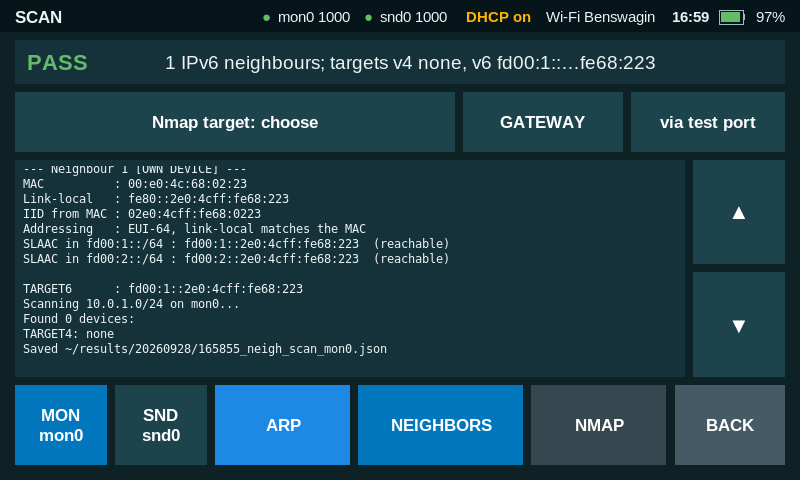
\includegraphics[width=0.72\textwidth]{Figures/gui_neighbours.png}
    \caption[Поиск соседей по IPv6 и сканирование ARP]{Поиск соседей: адреса, вычисленные по EUI-64 и проверенные тестом доступности; сканирование ARP без результата}
    \label{fig:gui_neighbours}
\end{figure}

\begin{table}[htbp]
    \caption{Поиск другой стороны на одном кабеле обоими протоколами}
    \label{tab:sousede}
    \centering
    \begin{tabular}{lll}
        \hline
        Протокол & Способ & Результат \\
        \hline
        IPv4 & сканирование ARP в диапазоне \texttt{10.0.1.0/24} & станций не найдено \\
        IPv6 & запрос на \texttt{ff02::1} и таблица соседей & сосед найден, адрес проверен \\
        \hline
    \end{tabular}
\end{table}

\subsection{Точность и пределы анализатора}
\label{sec:overeni_analyzatoru}

Точность анализатора проверена на перемычке между портами так: тот же процесс, что считал статистику, одновременно сохранял захваченный трафик в файл, который затем независимо пересчитан утилитой tcpdump с фильтрами по протоколам и утилитой capinfos. При смешанном трафике из ста ping по IPv4, ста ping по IPv6 и пятисекундной передачи TCP все счётчики совпали точно (таблица \ref{tab:presnost}). При передаче UDP со скоростью 10~Мбит/с в течение тридцати секунд анализатор насчитал 37\,503 датаграммы, а iperf3 отправил 37\,501 датаграмму без потерь; разница в две датаграммы — это два служебных сообщения, которыми iperf3 обменивается в начале теста. Разбор отдельных кадров на экране TRAFFIC дополнительно сравнён с утилитой tshark, то есть с разбором анализатора Wireshark: на 58 кадрах всех поддерживаемых типов совпали все 781 сравниваемое поле.

\begin{table}[htbp]
    \caption{Число кадров по протоколам: анализатор прибора и независимый пересчёт сохранённого файла}
    \label{tab:presnost}
    \centering
    \begin{tabular}{lrr}
        \hline
        Протокол & Анализатор прибора & Пересчёт tcpdump \\
        \hline
        TCP & 11\,251 & 11\,251 \\
        UDP & 0 & 0 \\
        ICMP & 200 & 200 \\
        ICMPv6 & 202 & 202 \\
        ARP & 4 & 4 \\
        всего & 11\,657 & 11\,657 \\
        \hline
    \end{tabular}
\end{table}

Предел анализатора искали, постепенно повышая скорость передачи UDP. Выразить его в мегабитах в секунду нельзя, потому что решает число кадров: обработка каждого кадра стоит одинаковой работы независимо от размера. С короткими кадрами размером 162~байта анализатор без потерь захватил 22\,498 кадров в секунду; при 26\,247 кадрах в секунду потерял уже 11,8~\%, а выше установился примерно на 23\,000 кадрах в секунду. Узкое место — одно ядро процессора, на котором идёт разбор заголовков и которое было загружено на 99~\%, тогда как у остальных ядер был запас. Для кадров полной длины 1514~байт этот предел соответствует примерно 270~Мбит/с, то есть примерно потолку шины USB 2.0: длинные кадры анализатор успевает, короткие на высокой скорости — нет.

Эффект фильтра в ядре измерен при передаче TCP со скоростью 50~Мбит/с с добавленными сообщениями ICMPv6. Без фильтра разбор загружал процессор на 27,2~\%, с фильтром \texttt{icmp6} — всего на 0,4~\%, и статистика содержала только сообщения ICMPv6. Кадры, не прошедшие фильтр, до программы действительно не доходили.

\subsection{Производительность генератора пакетов}
\label{sec:overeni_generatoru}

Генератор отправил тысячу сообщений ICMPv6 Echo Request со скоростью сто сообщений в секунду с порта \texttt{snd0}, и анализатор на порту \texttt{mon0} насчитал ровно тысячу (рисунок \ref{fig:gui_generator}); тот же результат дали все шесть поддерживаемых типов пакетов и обратное направление. Наибольшая скорость измерялась без захвата, по счётчику принятых кадров адаптера. С кадрами размером 100~байт генератор достиг 83\,764 кадров в секунду при загрузке одного ядра на 97~\%, с кадрами 1514~байт передал 157~Мбит/с при загрузке 17~\%, во всех случаях без потерь на приёмной стороне. Короткие кадры, таким образом, ограничивает процессор, длинные — шина. Смысл генератора при этом не в максимальной скорости: iperf3 с короткими датаграммами отправляет больше кадров в секунду, как показывает подраздел \ref{sec:mereni_propustnosti}. Генератор служит для отправки точно заданного числа пакетов определённого типа и проверки, что все они дошли.

\subsection{Измерение пропускной способности}
\label{sec:mereni_propustnosti}

Пропускная способность по TCP измерялась против ноутбука с обоих портов и обеими версиями IP. Результаты сведены в таблице \ref{tab:propustnost}, один из них показан на рисунке \ref{fig:gui_speed_tcp}. Все четыре измерения лежат между 273 и 276~Мбит/с и совпадают с измерением, проведённым ранее в лаборатории, где получилось 276~Мбит/с для IPv4 и 274~Мбит/с для IPv6. Разница между протоколами — единицы мегабит и соответствует более длинному заголовку IPv6, разобранному в разделе \ref{sec:ipv4_ipv6}.

\begin{table}[htbp]
    \caption{Пропускная способность по TCP, тест длительностью десять секунд}
    \label{tab:propustnost}
    \centering
    \begin{tabular}{llr}
        \hline
        Схема & Протокол & Пропускная способность [Мбит/с] \\
        \hline
        порт \texttt{mon0} против ноутбука & IPv4 & 274,0 \\
        порт \texttt{mon0} против ноутбука & IPv6 & 274,2 \\
        порт \texttt{snd0} против ноутбука & IPv4 & 273,3 \\
        порт \texttt{snd0} против ноутбука & IPv6 & 275,0 \\
        перемычка между портами & IPv6 & 150,5 \\
        \hline
    \end{tabular}
\end{table}

\begin{figure}[htbp]
    \centering
    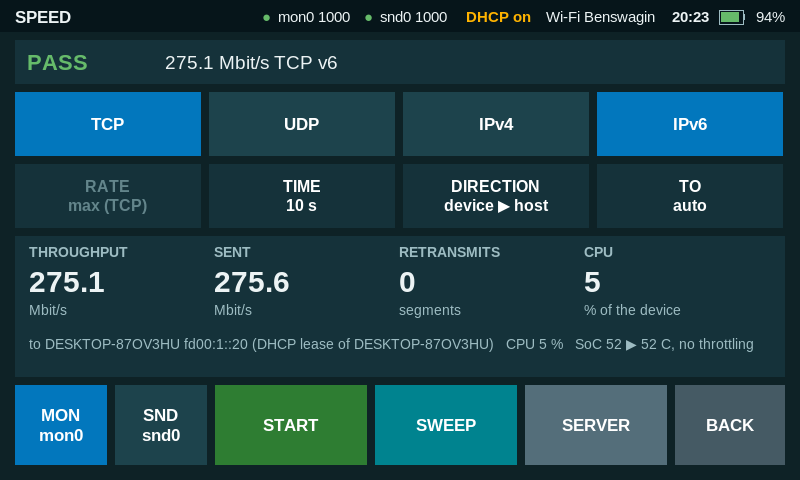
\includegraphics[width=0.72\textwidth]{Figures/gui_speed_tcp.png}
    \caption{Измерение пропускной способности по TCP и IPv6 против ноутбука}
    \label{fig:gui_speed_tcp}
\end{figure}

Значения лежат чуть ниже границы 300~Мбит/с, которую производитель указывает для Ethernet, подключённого через шину USB 2.0 \cite{rpi3bplus}. Измерение, таким образом, определило не пропускную способность линии, а потолок самого анализатора. На перемычке между портами потолок ещё примерно вдвое ниже, около 150~Мбит/с: каждый кадр проходит одну и ту же шину дважды — один раз при отправке одним адаптером и второй раз при приёме другим. Результаты с перемычки и с измерения против чужой станции поэтому смешивать нельзя. Прибор пригоден, чтобы проверить работоспособность соединения, сравнить протоколы и выявить грубые неисправности, но не для сертификации гигабитной линии на номинальной скорости.

Измерение по UDP со скоростью 100~Мбит/с прошло и против ноутбука в течение десяти секунд, и на перемычке в течение тридцати секунд без единой потерянной датаграммы, с джиттером 0,17~мс. При заданной скорости 400~Мбит/с, то есть выше возможностей платформы, прибор показал реально достигнутую скорость 265~Мбит/с, а не заданное значение.

Результаты развёртки по размерам кадра сведены в таблице \ref{tab:rozmitani} и на рисунке \ref{fig:graf_rozmitani}. Каждый размер измерялся десять секунд с отправкой настолько быстро, насколько мог прибор, и вся развёртка для каждого протокола заняла около 80 секунд (рисунок \ref{fig:gui_sweep}). Ход кривых показывает оба предела, о которых говорит теория. На коротких кадрах прибор отправляет до 147 тысяч кадров в секунду, но пропускная способность низкая, потому что процессор отправляющего инструмента загружен полностью. С ростом размера кадра число кадров падает, а пропускная способность по кадрам приближается к 276~Мбит/с, то есть к потолку шины. Потери не более 1,4~\% появлялись только на некоторых коротких кадрах и менялись от измерения к измерению, потому что возникали на приёмной стороне.

\begin{table}[htbp]
    \caption{Развёртка по размерам кадра по UDP, анализатор против ноутбука}
    \label{tab:rozmitani}
    \centering
    \begin{tabular}{rrrrrr}
        \hline
        & \multicolumn{2}{c}{IPv4} & & \multicolumn{2}{c}{IPv6} \\
        Кадр [Б] & Мбит/с & тыс. кадров/с & Кадр [Б] & Мбит/с & тыс. кадров/с \\
        \hline
        64 & 67,1 & 131,1 & 82 & 81,2 & 123,8 \\
        128 & 150,5 & 147,0 & 128 & 137,1 & 133,9 \\
        256 & 224,6 & 109,7 & 256 & 224,0 & 109,4 \\
        512 & 247,4 & 60,4 & 512 & 246,8 & 60,3 \\
        1024 & 268,5 & 32,8 & 1024 & 269,8 & 32,9 \\
        1280 & 273,6 & 26,7 & 1280 & 272,1 & 26,6 \\
        1518 & 276,4 & 22,8 & 1518 & 276,5 & 22,8 \\
        \hline
    \end{tabular}
\end{table}

\begin{figure}[htbp]
    \centering
    % Развёртка UDP по размеру кадра (русская версия рис. 3.13)
\begin{tikzpicture}
    \begin{axis}[
        width=0.8\textwidth, height=6.2cm,
        xmode=log, log basis x=2,
        xtick={64,128,256,512,1024,1518}, xticklabels={64,128,256,512,1024,1518},
        xlabel={размер кадра [Б]},
        ylabel={пропускная способность по кадрам [Мбит/с]},
        ymin=0, ymax=300,
        axis y line*=left,
        legend style={at={(0.5,-0.28)}, anchor=north, legend columns=2, font=\footnotesize, draw=none},
        grid=major, grid style={gray!25},
        tick label style={font=\footnotesize}, label style={font=\small}]
        \addplot[thick, mark=*, mark size=1.6pt] table[x=frame, y=frame_mbps] {../Figures/data/sweep_v4.csv};
        \addlegendentry{IPv4, Мбит/с}
        \addplot[thick, mark=square*, mark size=1.6pt, gray] table[x=frame, y=frame_mbps] {../Figures/data/sweep_v6.csv};
        \addlegendentry{IPv6, Мбит/с}
        \addlegendimage{thick, dashed, mark=o}
        \addlegendentry{IPv4, тыс. кадров/с}
        \addlegendimage{thick, dashed, mark=square, gray}
        \addlegendentry{IPv6, тыс. кадров/с}
    \end{axis}
    \begin{axis}[
        width=0.8\textwidth, height=6.2cm,
        xmode=log, log basis x=2,
        xtick=\empty,
        ylabel={кадров в секунду [тысячи]},
        ymin=0, ymax=160,
        axis y line*=right, axis x line=none,
        tick label style={font=\footnotesize}, label style={font=\small}]
        \addplot[thick, dashed, mark=o, mark size=1.6pt] table[x=frame, y=kpps] {../Figures/data/sweep_v4.csv};
        \addplot[thick, dashed, mark=square, mark size=1.6pt, gray] table[x=frame, y=kpps] {../Figures/data/sweep_v6.csv};
    \end{axis}
\end{tikzpicture}

    \caption[Пропускная способность и кадры в секунду в зависимости от размера кадра]{Пропускная способность по кадрам и число кадров в секунду в зависимости от размера кадра}
    \label{fig:graf_rozmitani}
\end{figure}

\begin{figure}[htbp]
    \centering
    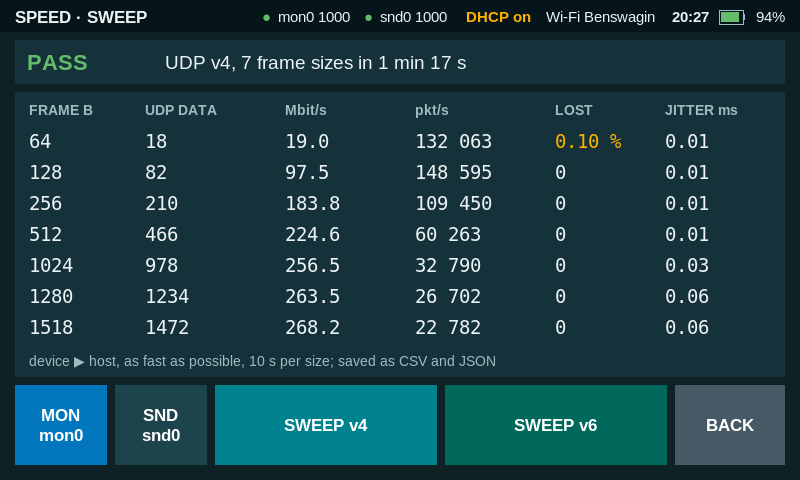
\includegraphics[width=0.72\textwidth]{Figures/gui_sweep.png}
    \caption{Результат развёртки по размерам кадра на дисплее прибора}
    \label{fig:gui_sweep}
\end{figure}

Режим сервера проверен так: измерение против прибора запускал ноутбук (рисунок \ref{fig:gui_server}). Прибор принял 249~Мбит/с по TCP, а в обратном направлении отправил 272~Мбит/с. После нажатия STOP в пространстве имён порта не осталось ни одного процесса сервера.

\begin{figure}[htbp]
    \centering
    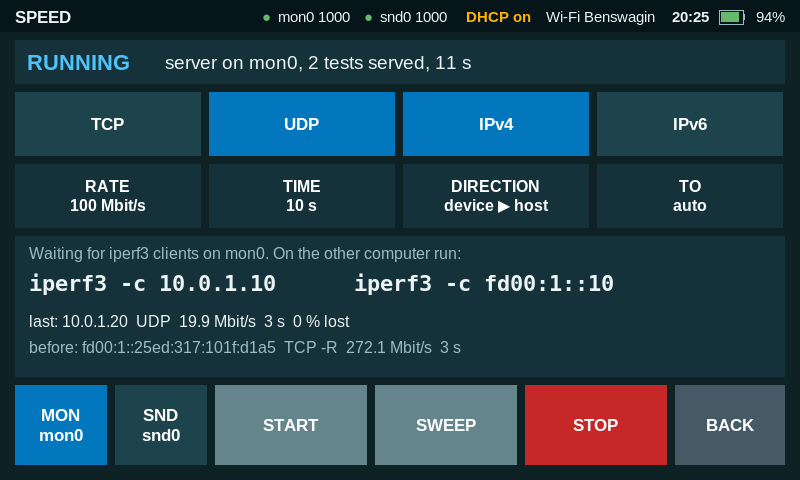
\includegraphics[width=0.72\textwidth]{Figures/gui_server.png}
    \caption{Режим сервера: ноутбук измеряет пропускную способность против анализатора}
    \label{fig:gui_server}
\end{figure}

\subsection{Подключение обычного компьютера}
\label{sec:overeni_notebook}

Ноутбук с Windows 11 получил от прибора на обоих адаптерах адреса \texttt{10.0.1.20} и \texttt{10.0.2.20}, а для IPv6 — по три адреса: выданный DHCPv6, составленный автоконфигурацией с идентификатором, не выведенным из физического адреса, и вдобавок временный адрес. Маршрута по умолчанию через анализатор не появилось, и ноутбук остался подключён к Интернету через Wi-Fi, что подтвердило правильность решения из подраздела \ref{sec:architektura}.

Первый ping остался без ответа. Windows считает неизвестную сеть общественной и блокирует на ней входящие сообщения Echo Request; на сообщения, отправленные на групповой адрес всех узлов, не отвечает вовсе. При этом прибор правильно сообщил, что станция подключена, поскольку она ответила на запрос ARP и Neighbor Solicitation, и что ping блокирует её межсетевой экран. После разрешения входящих Echo Request на обоих тестовых адаптерах тесты во всех четырёх сочетаниях порта и протокола прошли без потерь с временем отклика от 1,2 до 1,8~мс.

Измерение по UDP поверх IPv6 поначалу не удавалось установить. Журнал сервера iperf3 на ноутбуке показал, что сервер отвечает со своего временного адреса, хотя анализатор посылал запрос на адрес, выданный DHCPv6. Временные адреса служат защите приватности, и система предпочитает их при отправке \cite{rfc8981}; не привязанный к адресу сервер iperf3 поэтому ответил не с того адреса, к которому к нему обратились, и анализатор такой ответ законно отбросил. После запуска сервера с привязкой к конкретному адресу измерение прошло без ошибок. Теперь в такой ситуации прибор показывает объяснение и рекомендацию.

Самым важным выводом стало поведение передачи UDP в обратном направлении, то есть с ноутбука в анализатор. При 20~Мбит/с потерь почти не было, при 50~Мбит/с они составили 24~\%, при 100~Мбит/с — 57~\%, хотя в том же направлении TCP передал 250~Мбит/с. Буфер сокета на анализаторе не переполнялся, а ноутбук по своим счётчикам отправил все датаграммы. Решил дело счётчик пропущенных кадров адаптера: за одно измерение он вырос на 13\,559, а iperf3 насчитал 13\,543 потерянные датаграммы. Кадры, таким образом, выбрасывает сам адаптер анализатора. iperf3 в Windows выдерживает заданную среднюю скорость, но отправляет датаграммы пачками на полной скорости гигабитной линии, и адаптер на шине USB 2.0 не успевает передать их дальше. TCP приспосабливается к этому управлением потоком, UDP — нет. Это реальный предел прибора как приёмника: пачечный трафик со скоростью выше пропускной способности шины теряется уже на входе. Поэтому прибор теперь записывает значение этого счётчика к каждому измерению и объясняет, где произошла потеря.

\subsection{Питание и время автономной работы}
\label{sec:overeni_napajeni}

Время автономной работы измерено разрядным тестом в типичном режиме, то есть с пассивным прослушиванием на порту мониторинга, включённым дисплеем и подключённой сетью Wi-Fi. Прибор проработал от полностью заряженного аккумулятора 6 часов 43 минуты, пока напряжение ячеек не упало ниже 9,6~В и служба штатно его не выключила (рисунок \ref{fig:graf_vybijeni}). Аккумулятор за это время отдал 2,51~А·ч и 28,2~Вт·ч, то есть 84~\% номинальной ёмкости ячеек, при среднем потреблении 4,2~Вт. Напряжение падало почти равномерно, кроме последних получаса, когда оно падало вдвое быстрее. Худший случай из таблицы \ref{tab:spotreba} отдельно не измерялся; из той же энергии и большего потребления получается оценка около четырёх часов.

\begin{figure}[htbp]
    \centering
    % Разрядный тест аккумулятора (русская версия рис. 3.16)
\begin{tikzpicture}
    \begin{axis}[
        width=0.8\textwidth, height=5.8cm,
        xlabel={время работы от аккумулятора [ч]},
        ylabel={напряжение последовательных ячеек [В]},
        xmin=0, xmax=7, ymin=9.4, ymax=12.6,
        xtick={0,1,2,3,4,5,6,7},
        grid=major, grid style={gray!25},
        tick label style={font=\footnotesize}, label style={font=\small}]
        \addplot[thick] table[x=h, y=v] {../Figures/data/discharge.csv};
        \draw[dashed] (axis cs:0,9.6) -- (axis cs:7,9.6);
        \node[anchor=south west, font=\footnotesize] at (axis cs:0.1,9.6) {порог отключения 9,6 В};
        \node[anchor=south west, font=\footnotesize, align=left] at (axis cs:0.3,10.05) {отключение через 6~ч 43~мин\\отдано 28,2~Вт·ч};
    \end{axis}
\end{tikzpicture}

    \caption{Напряжение аккумулятора во время разрядного теста в типичном режиме}
    \label{fig:graf_vybijeni}
\end{figure}

По той же записи построена кривая, по которой прибор переводит напряжение в оставшийся заряд в процентах и оценивает оставшееся время работы. Отдельно измерено, что даёт блокировка экрана: выключение выхода HDMI снизило потребление от аккумулятора с 4,53 до 4,18~Вт, то есть на 0,35~Вт, что продлит работу заблокированного прибора примерно на полчаса. Выключение линий тестовых портов потребление не снизило вовсе.

\subsection{Сканирование сети и проверка изоляции пространств имён}
\label{sec:skenovani}

Сканер Nmap запускается с экрана SCAN — либо через тестовый порт внутри его пространства имён, либо через интерфейс Wi-Fi с автоматической подстановкой шлюза по умолчанию беспроводной сети. На рисунке \ref{fig:gui_nmap_lan} показано сканирование второго порта того же прибора через перемычку. Сканер нашёл станцию, определил производителя её адаптера по физическому адресу и установил, что из ста самых распространённых портов не открыт ни один; прибор, таким образом, не выставляет на своих тестовых портах никаких служб.

\begin{figure}[htbp]
    \centering
    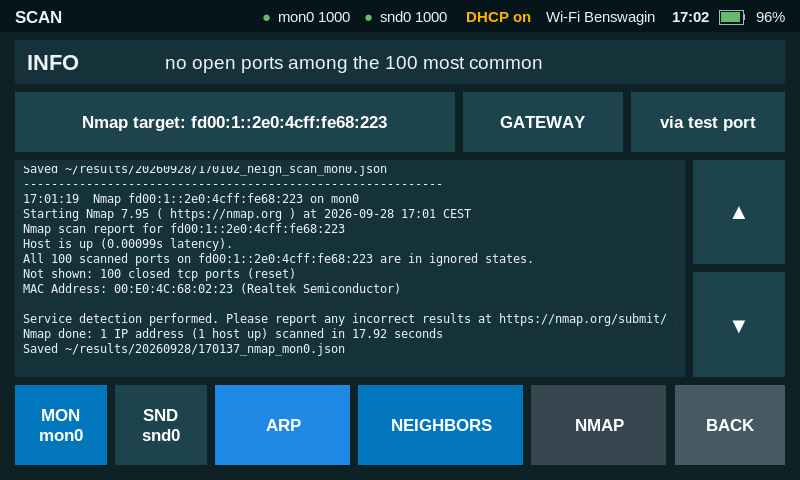
\includegraphics[width=0.72\textwidth]{Figures/gui_nmap_lan.png}
    \caption{Сканирование Nmap через тестовый порт}
    \label{fig:gui_nmap_lan}
\end{figure}

Проверка сканера выявила и дефект первой версии приложения, который одновременно служит доказательством изоляции. В режиме проводного сканирования сканер жёстко запускался в пространстве имён \texttt{analyzer\_sender}, поэтому попытка сканировать адрес \texttt{10.0.1.20} из подсети порта мониторинга заканчивалась сообщением \texttt{failed to determine route}. Тот же адрес из пространства \texttt{analyzer\_monitor} был доступен без проблем. Это была не неисправность сети, а следствие того, что между пространствами намеренно нет пути: трафик из одного пространства не попадёт в другое, даже если об этом прямо попросить. Инструменты теперь всегда запускаются в пространстве имён порта, выбранного на экране.

\subsection{Дефекты, выявленные при повторной проверке}
\label{sec:odhalene_vady}

Повторная проверка выявила несколько дефектов, которые не проявились при первом проходе измерений и могли остаться скрытыми до применения прибора вне лаборатории.

Самый серьёзный касался исходного счётчика трафика. Он различал протоколы по словам в текстовом выводе tcpdump, но строки с сегментами TCP слова «TCP» не содержат. При контрольном измерении счётчик насчитал ноль сегментов TCP, тогда как одновременно сохранённый файл содержал их 1202; счётчики UDP и ICMP при этом были верны. Дефект устранён заменой счётчика анализатором из подраздела \ref{sec:analyzator}, который читает двоичные заголовки.

Скрипт инициализации при повторном запуске в том же сеансе системы давал сбой, потому что пытался перенести интерфейс в новое пространство имён раньше, чем ядро после удаления старого пространства вернуло его в основное. Дефект исчез с переходом на службу, которая пространства заново не создаёт, а только достраивает недостающее.

Ещё один дефект управляющего приложения был обнаружен способом, заслуживающим упоминания. На снимке экрана лента выглядела прерывистой, часть текста дублировалась, хотя содержимое ленты, прочитанное программно, было безупречным. Причина была в том, что отдельные задачи писали в элементы интерфейса прямо из своих потоков, чего использованная библиотека не допускает и что в крайнем случае ведёт к падению приложения. Запись в элементы интерфейса теперь откладывается в главный поток.

Два меньших дефекта выявило только подключение реального компьютера и съёмка экранов для этой работы. Записи об адресах, выданных DHCP, живут двенадцать часов, и прибор после отключения ноутбука пытался обратиться к станции, которой уже не было; кандидаты в цели теперь проверяются заново. Сканер Nmap, не успевший исследовать станцию за заданный лимит времени, оценивался как сканирование без открытых портов; теперь такое сканирование оценивается как незавершённое. Общий урок: то, что на дисплее, нужно сверять с независимо полученными данными, а не полагаться на то, что видно.

\chapter{Заключение}
\label{sec:zaver}

Цель этой бакалаврской работы — спроектировать и реализовать переносное устройство для тестирования и мониторинга компьютерных сетей, которое содержит генератор и анализатор трафика протоколов IPv4 и IPv6 и позволяет измерять такие параметры сети, как задержка, пропускная способность и потери. Эта цель достигнута.

В теоретической части описана проблематика генерирования сетевого трафика, включая разницу между измерением в битах и в кадрах в секунду, рекомендуемые размеры кадра и расчёт джиттера, и проблематика мониторинга сетей, включая фильтрацию трафика в ядре, сводные статистики и пределы самого захвата. Кроме того, разобраны адресация и автоконфигурация протокола IPv6 и технология пространств имён, на которой построен прибор.

В практической части создан прототип на основе одноплатного компьютера Raspberry Pi с сенсорным дисплеем, двумя внешними сетевыми адаптерами и аккумуляторным модулем. После включения прибор сразу запускает управляющее приложение и в типичном режиме работает от аккумулятора 6 часов 43 минуты. Он содержит анализатор трафика со сводными статистиками, разбором отдельных кадров, фильтрами в ядре и сохранением в формат pcap, генератор пакетов шести типов, измерение задержки тестом ping и измерение пропускной способности, потерь и джиттера инструментом iperf3, включая развёртку по размерам кадра и режим сервера. Для IPv6 он предлагает аудит сообщений Router Advertisement и поиск соседей с вычислением их адресов.

Решение проверено измерениями — и на перемычке между двумя портами прибора, и против чужой станции под Linux, и против ноутбука под Windows. Анализатор насчитал столько же кадров, сколько независимый пересчёт сохранённого файла, и его разбор совпал с анализатором Wireshark. Генератор доставил все отправленные пакеты во второе пространство имён. Пропускная способность по TCP против ноутбука составила 273--276~Мбит/с для обоих протоколов IP.

\section*{Собственный вклад автора}
\addcontentsline{toc}{section}{Собственный вклад автора}

Первый вклад — архитектура прибора, в которой оба тестовых интерфейса логически разделены пространствами имён ядра Linux, а каждая измерительная функция — отдельный скрипт, который работает в пространстве выбранного порта и передаёт результат управляющему приложению в машиночитаемом виде. Разделение устраняет конфликты маршрутизации между двумя интерфейсами в одном сегменте и проверено измерением: попытка обратиться к цели из неправильного пространства заканчивается недоступностью маршрута, а пакеты генератора попадают во второе пространство только по кабелю. Каждый результат сохраняется вместе со временем и контрольной суммой использованного скрипта, так что его происхождение можно проследить.

Второй вклад — разбор автоконфигурации адресов IPv6 на стороне анализатора. Показано, что dnsmasq при диапазоне, заданном одним адресом, опускает у объявленного префикса флаг A, и что после добавления ключевого слова \texttt{slaac} ядро станции само составляет адрес без какого-либо процесса в пространстве пользователя; контрольный порт с исходной настройкой подтвердил, что другая причина на результат не влияла. На этот разбор опирается модуль аудита, который разбирает сообщение Router Advertisement, оценивает его по требованиям стандартов и различает отправку собственного порта, второго порта того же прибора и чужого маршрутизатора, а также поиск соседей, который на одном и том же кабеле показал, что IPv6 находит другую сторону там, где IPv4 не находит ничего.

Третий вклад — пара генератора и анализатора трафика с проверенной точностью и измеренными пределами. Анализатор без потерь захватывает около 22\,500 кадров в секунду, генератор отправляет до 84\,000 кадров в секунду, и оба предела задаются производительностью процессора, а не объёмом данных. Измерения показали также, что на перемычке между портами пропускная способность вдвое ниже, потому что каждый кадр проходит шину USB дважды, и что адаптер прибора выбрасывает кадры UDP, если они приходят пачками быстрее, чем шина успевает их передать. Эти выводы определяют, как толковать измеренные числа.

Четвёртый вклад — воплощение устройства как самостоятельного прибора. Он работает от собственного аккумулятора с измерением заряда и штатным выключением при разряде, управляется пальцем на резистивном дисплее с элементами управления, рассчитанными на касание, и после подключения к чужой сети сам ничего не отправляет. Подключённой станции он выдаёт только адрес, а не шлюз по умолчанию, поэтому не нарушает её существующее подключение к Интернету. Для не прошедших тестов он объясняет оператору причину и советует, что делать дальше.

\section*{Ограничения и рекомендации по дальнейшему развитию}
\addcontentsline{toc}{section}{Ограничения и рекомендации по дальнейшему развитию}

Границы прибора нужно очертить честно. Ethernet использованной платформы подключён через шину USB 2.0, поэтому прибор достигает не более примерно 276~Мбит/с; он пригоден, чтобы проверить работоспособность соединения, сравнить протоколы в одинаковых условиях и выявить грубые неисправности, но не для сертификации гигабитной линии. Устранение этого ограничения потребовало бы перехода на более новое поколение одноплатного компьютера с контроллером Ethernet не на шине USB. Это же касается приёма пачечного трафика UDP и предела анализатора в кадрах в секунду.

Для дальнейшего развития есть несколько направлений. Ближайшее — корпус, в котором все компоненты будут жёстко закреплены; прибор уже работает от аккумулятора, но его части пока соединены свободно. Второе направление — автоматический тест розетки одной кнопкой, который после подключения к сети проверил бы линию, доступность сервера DHCP и маршрутизатора IPv6, шлюз по умолчанию и разрешение имён, как это делают коммерческие тестеры. Далее — определение свойств порта, то есть согласованной скорости, данных протоколов обнаружения соседних устройств и меток VLAN, затем определение наибольшего размера пакета, проходящего по пути, экспорт результатов на носитель и уточнение сенсорного управления калибровкой резистивной панели. Модуль аудита IPv6 подсказывает и направление безопасности: проверки, отработанные в этой работе на намеренно испорченном сообщении, в рабочей сети смогли бы обнаружить неправильно настроенный или несанкционированно подключённый маршрутизатор.


\printbibliography[title={Литература}, heading=bibintoc]

\appendix
\chapter{Исходные коды измерительных скриптов}
\label{sec:Appendix1}

В оригинале работы (приложение A) напечатаны исходные коды семи ключевых скриптов: \texttt{setup\_network.sh}, \texttt{sniff\_stats.py}, \texttt{pkt\_gen.py}, \texttt{perf\_test.py}, \texttt{ra\_audit.py}, \texttt{neigh\_scan.py} и \texttt{arp\_scan.py}. В этом переводе коды не повторяются: они одинаковы в обеих версиях и лежат в папке \texttt{SourceCodes/} проекта.

\chapter{Обзор программного обеспечения прибора}
\label{sec:Appendix2}

Программное обеспечение хранится в каталоге \texttt{\textasciitilde/diploma\_project/} на карте памяти прибора; системные файлы лежат в обычных местах системы. Полные исходные коды всех файлов входят в электронное приложение к работе. Обзор приведён в таблице \ref{tab:soubory}; скрипты, напечатанные в приложении A оригинала, отмечены звёздочкой.

\begin{table}[htbp]
    \caption{Файлы программного обеспечения прибора}
    \label{tab:soubory}
    \centering
    \small
    \begin{tabular}{lp{9.5cm}}
        \hline
        Файл & Назначение \\
        \hline
        \multicolumn{2}{l}{\textit{Измерительные скрипты, запускаются в пространстве имён порта}} \\
        \texttt{setup\_network.sh}* & подготовка портов, пространств имён и сервера dnsmasq \\
        \texttt{sniff\_stats.py}* & анализатор трафика, статистика, сохранение в pcap и CSV \\
        \texttt{pktdecode.py} & разбор заголовков кадра без Scapy, для статистики и для разбора по слоям \\
        \texttt{pkt\_gen.py}* & генератор пакетов шести типов \\
        \texttt{perf\_test.py}* & измерения iperf3 и развёртка по размерам кадра \\
        \texttt{perf\_server.py} & сервер iperf3 на выбранном порту \\
        \texttt{path\_test.py} & тест доступности и задержки утилитой ping \\
        \texttt{targets.py} & общий поиск цели и объяснение, почему цели нет \\
        \texttt{ra\_audit.py}* & аудит сообщений Router Advertisement \\
        \texttt{neigh\_scan.py}* & поиск соседей IPv6 \\
        \texttt{arp\_scan.py}* & сканирование ARP \\
        \multicolumn{2}{l}{\textit{Управляющее приложение}} \\
        \texttt{gui\_app.py} & главный экран, запуск задач, экран приветствия и блокировки \\
        \texttt{ui\_kit.py} & общий вид экранов, строка состояния, кнопки \\
        \texttt{screens.py} & экраны PATH, SCAN, IPv6, DHCP / RA и SYSTEM \\
        \texttt{traffic.py} & экран TRAFFIC с разбором кадра и фильтрами \\
        \texttt{generator.py} & экран GENERATOR \\
        \texttt{speed.py} & экран SPEED с развёрткой и режимом сервера \\
        \texttt{results.py} & сохранение результатов в файлы JSON \\
        \texttt{wifi\_dialog.py} & подключение к сети Wi-Fi и клавиатура на экране \\
        \multicolumn{2}{l}{\textit{Системные службы}} \\
        \texttt{port\_status.py} & слежение за состоянием портов и запись в файл состояния \\
        \texttt{ups\_monitor.py} & измерение состояния аккумулятора и штатное выключение при разряде \\
        \texttt{analyzer-port@.service} & подготовка порта при подключении адаптера \\
        \texttt{10-analyzer-*.link} & постоянные имена портов по физическому адресу \\
        \texttt{\textasciitilde/.xinitrc} & запуск управляющего приложения вместо рабочего стола \\
        \hline
    \end{tabular}
\end{table}


\end{document}
